\section{Casi d'uso}
Di seguito sono riportati i casi d'uso per l'individuazione dei requisiti funzionali.\\
Le convenzioni utilizzate per etichettare i casi d'uso sono quelle riportate nelle \emph{\NormeDiProgetto} (cap. 7).\\
\subsection{Gerarchia utenti}
In tutti i casi d'uso sia considerata valida la seguente gerarchia di utenti:

\begin{figure}[htbp]
\centering
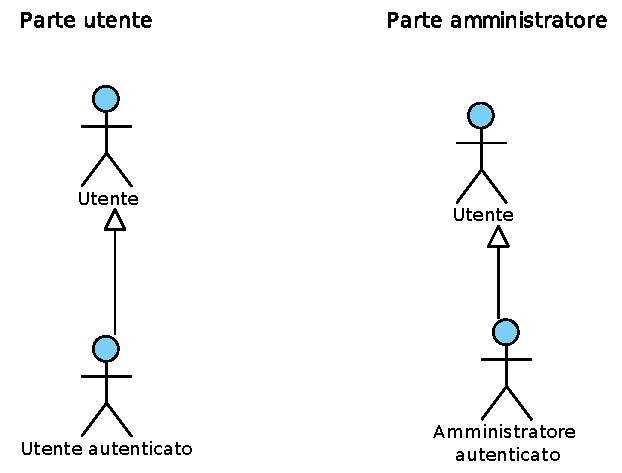
\includegraphics[scale=0.7]{./casi_uso/Utenti.pdf}
\label{figUtenti}
\caption{Gerarchia utenti.}
\end{figure}


\newpage

\subsection{Ambito utente}
\subsubsection{UC 0 Caso base utente}
\label{sec:UC0generale}

\begin{figure}[htbp]
\centering
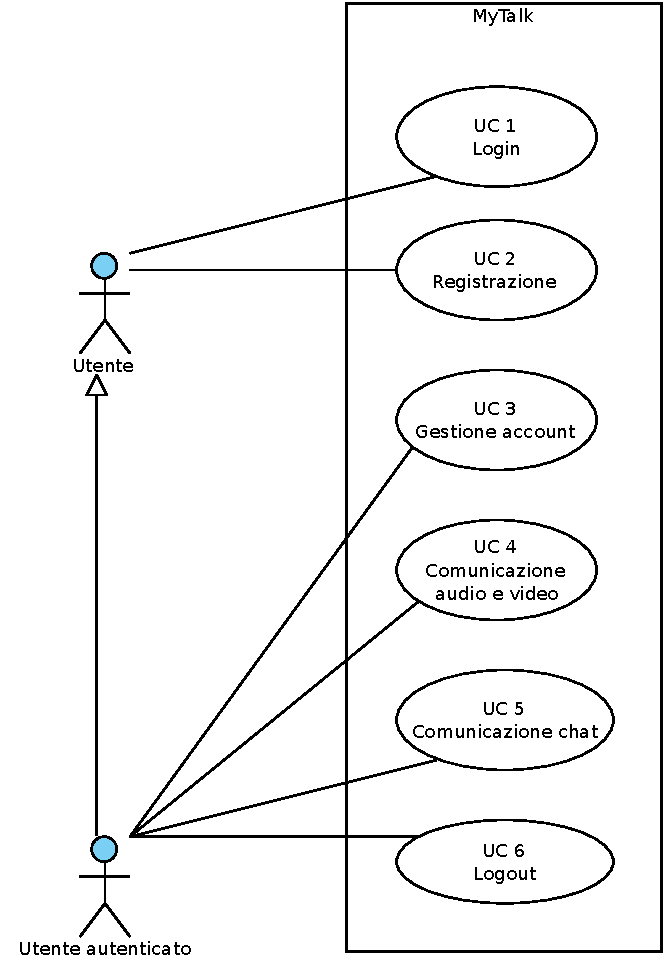
\includegraphics[scale=0.7]{./casi_uso/UC0.pdf}
\label{figUC0}
\caption{UC 0 Caso base utente.}
\end{figure}

\noindent
\textbf{Attori primari:} Utente, utente autenticato.\\
\textbf{Descrizione:} l'utente appena entrato nel sito risulta essere non autenticato, può quindi registrarsi oppure se è già registrato può effettuare il login diventando utente autenticato. L'utente autenticato può chiamare ed essere chiamato da altri utenti registrati, comunicare tramite chat, gestire il proprio account ed effettuare il logout diventando nuovamente utente.\\
\textbf{Precondizione:}  il sistema è funzionante e pronto all'utilizzo, l'utente è entrato nel sito del sistema.\\
\textbf{Postcondizione:} l'utente ha effettuato le operazioni che desiderava, eventuali registrazioni, modifiche e altre operazioni sono state eseguite e/o salvate dal sistema.\\
\textbf{Scenario principale:}
\begin{itemize}
\item l'utente può effettuare la registrazione;
\item l'utente può effettuare il login diventando utente autenticato;
\item l'utente autenticato può effettuare e ricevere video chiamate;
\item l'utente autenticato può comunicare tramite chat;
\item l'utente autenticato può gestire il proprio account;
\item l'utente autenticato può effettuare il logout, ridiventando utente.
\end{itemize} 

\subsubsection{UC 1 Login}

\begin{figure}[htbp]
\centering
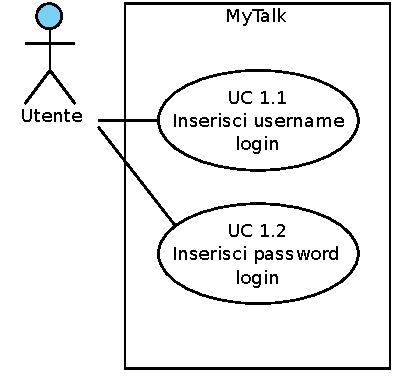
\includegraphics[scale=0.7]{./casi_uso/UC1.pdf}
\caption{UC 1 Login utente.}
\end{figure}

\noindent
\textbf{Attori primari:} utente, utente autenticato.\\
\textbf{Descrizione:} l'utente inserisce il proprio username e la propria password, se queste risultano corrette l'utente viene autenticato.\\
\textbf{Precondizione:} il sistema è funzionante e l'utente non ancora autenticato vuole effettuare il login.\\
\textbf{Postcondizione:} l'utente è autenticato, diventa quindi utente autenticato ed entra nel sistema, il sistema è funzionante e può permettere all'utente autenticato di comunicare e gestire il proprio account.\\
\textbf{Scenario principale:}
\begin{itemize}
\item l'utente inserisce il proprio username;
\item l'utente inserisce la propria password;
\item avviene l'autenticazione;
\end{itemize}					
\textbf{Scenario alternativo:} le credenziali non risultano essere corrette e viene data opportuna comunicazione all'utente che avrà eventualmente la possibilità di reinserire i dati.\\

\subsubsection{UC 1.1 Inserisci username login}
\noindent
\textbf{Attori primari:} utente.\\
\textbf{Descrizione:} l'utente immette il proprio username.\\
\textbf{Precondizione:} l'utente è pronto ad inserire il proprio username per il login.\\
\textbf{Postcondizione:} l'utente ha immesso il proprio username.\\
\textbf{Scenario principale:}
\begin{itemize}
\item l'utente immette il proprio username.
\end{itemize}

\subsubsection{UC 1.2 Inserisci password login}
\noindent
\textbf{Attori primari:} utente.\\
\textbf{Descrizione:} l'utente immette la propria password.\\
\textbf{Precondizione:} l'utente è pronto ad inserire la propria password per il login.\\
\textbf{Postcondizione:} l'utente ha immesso la propria password.\\
\textbf{Scenario principale:}
\begin{itemize}
\item l'utente immette la propria password.
\end{itemize}

\subsubsection{UC 2 Registrazione}

\begin{figure}[htbp]
\centering
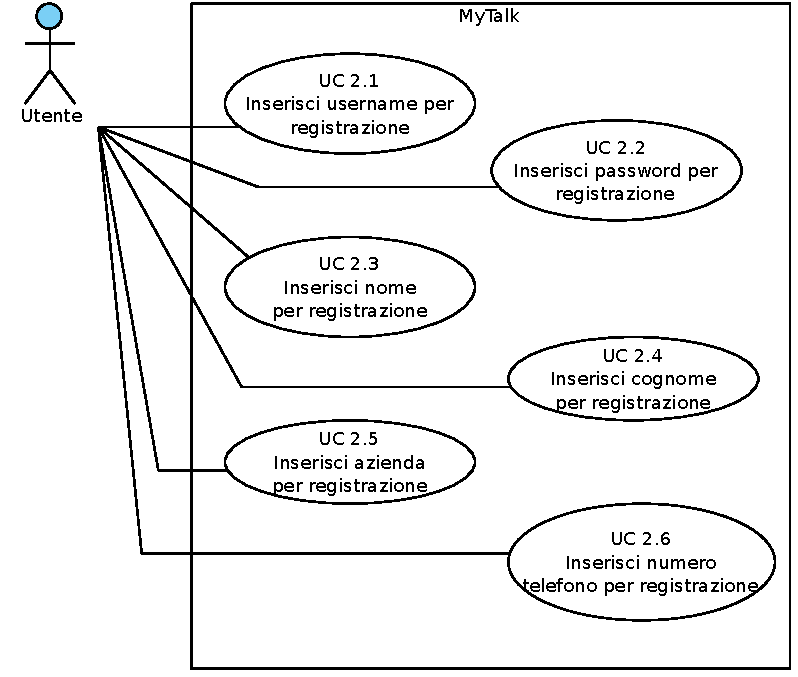
\includegraphics[scale=0.7]{./casi_uso/UC2.pdf}
\caption{UC 2 Registrazione nuovo utente.}
\end{figure}

\noindent
\textbf{Attori primari:} utente.\\
\textbf{Descrizione:} l'utente vuole registrarsi nel sistema, inserisce quindi i suoi dati e dopo aver ricevuto conferma dal sistema viene registrato.\\
\textbf{Precondizione:} il sistema è funzionante e l'utente richiede la registrazione.\\
\textbf{Postcondizione:} la registrazione è stata effettuata, il sistema ha salvato i dati immessi dall'utente ed ora è al punto iniziale  (figura: \ref{figUC0}).\\
\textbf{Scenario principale:}
\begin{itemize}
\item l'utente inserisce lo username scelto;
\item l'utente inserisce la password scelta;
\item l'utente inserisce il proprio nome;
\item l'utente inserisce il proprio cognome;
\item l'utente, a sua discrezione, inserisce l'azienda in cui lavora;
\item l'utente, a sua discrezione, inserisce il proprio numero di telefono;
\item l'utente viene registrato;
\end{itemize}
\textbf{Scenario alternativo:} lo username scelto risulta essere appartenente ad un altro utente, l'utente che si sta registrando viene avvisato dell'errore e può scegliere un altro username.\\
\textbf{Scenario alternativo:} la password e la sua conferma risultano essere diverse, l'utente viene avvisato dell'errore e può reinserire i dati.

\subsubsection{UC 2.1 Inserisci username per registrazione}
\noindent
\textbf{Attori primari:} utente.\\
\textbf{Descrizione:} l'utente inserisce il proprio username.\\
\textbf{Precondizione:} l'utente richiede la registrazione e vuole procedere con l'inserimento dello username scelto.\\
\textbf{Postcondizione:} lo username è stato inserito, il sistema procede con la procedura di registrazione.\\
\textbf{Scenario principale:}
\begin{itemize}
\item l'utente inserisce lo username da lui scelto;
\end{itemize}

\subsubsection{UC 2.2 Inserisci password per registrazione}
\noindent
\textbf{Attori primari:} utente.\\
\textbf{Descrizione:} l'utente inserisce la propria password.\\
\textbf{Precondizione:} l'utente richiede la registrazione e vuole procedere con l'inserimento della password.\\
\textbf{Postcondizione:} la password è stata inserita, il sistema procede con la procedura di registrazione.\\
\textbf{Scenario principale:}
\begin{itemize}
\item l'utente inserisce la password da lui scelta.
\end{itemize}

\subsubsection{UC 2.3 Inserisci nome per registrazione}
\noindent
\textbf{Attori primari:} utente.\\
\textbf{Descrizione:} l'utente inserisce il proprio nome.\\
\textbf{Precondizione:} l'utente richiede la registrazione e vuole procedere con l'inserimento del proprio nome.\\
\textbf{Postcondizione:} il nome è stato inserito, il sistema procede con la procedura di registrazione.\\
\textbf{Scenario principale:}
\begin{itemize}
\item l'utente inserisce il proprio nome.
\end{itemize}

\subsubsection{UC 2.4 Inserisci cognome per registrazione}
\noindent
\textbf{Attori primari:} utente.\\
\textbf{Descrizione:} l'utente inserisce il proprio cognome.\\
\textbf{Precondizione:} l'utente richiede la registrazione e vuole procedere con l'inserimento del proprio cognome.\\
\textbf{Postcondizione:} il cognome è stato inserito, il sistema procede con la procedura di registrazione.\\
\textbf{Scenario principale:}
\begin{itemize}
\item l'utente inserisce il proprio cognome.
\end{itemize}

\subsubsection{UC 2.5 Inserisci azienda per registrazione}
\noindent
\textbf{Attori primari:} utente.\\
\textbf{Descrizione:} l'utente inserisce l'azienda per cui attualmente lavora.\\
\textbf{Precondizione:} l'utente richiede la registrazione e procede con l'inserimento della propria azienda.\\
\textbf{Postcondizione:} l'azienda è stata inserita, il sistema procede con la procedura di registrazione.\\
\textbf{Scenario principale:}
\begin{itemize}
\item l'utente inserisce l'azienda per cui lavora.
\end{itemize}
\textbf{Scenario alternativo:} l'utente si rifiuta di inserire l'azienda per cui lavora, il sistema prosegue ugualmente con la registrazione ignorando l'azienda che è quindi opzionale.\\

\subsubsection{UC 2.6 Inserisci numero di telefono per registrazione}
\noindent
\textbf{Attori primari:} utente.\\
\textbf{Descrizione:} l'utente inserisce il proprio numero di telefono.\\
\textbf{Precondizione:} l'utente richiede la registrazione e procede con l'inserimento del proprio numero di telefono.\\
\textbf{Postcondizione:} il numero di telefono è stato inserito, il sistema procede con la procedura di registrazione.\\
\textbf{Scenario principale:}
\begin{itemize}
\item l'utente inserisce il proprio numero di telefono.
\end{itemize}
\textbf{Scenario alternativo:} l'utente si rifiuta di inserire il proprio numero di telefono, il sistema prosegue ugualmente con la registrazione ignorando il numero di telefono che è quindi opzionale.\\


\subsubsection{UC 3 Gestione account}

\begin{figure}[htbp]
\centering
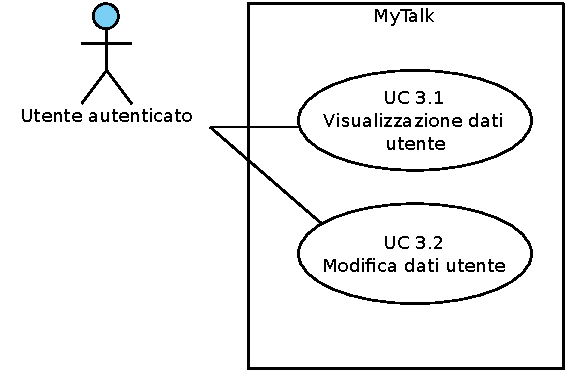
\includegraphics[scale=0.7]{./casi_uso/UC3.pdf}
\caption{UC 3 Gestione account utente.}
\end{figure}

\noindent
\textbf{Attori primari:} utente autenticato.\\
\textbf{Descrizione:} l'utente visualizza i suoi dati ed, eventualmente, può modificarli.\\
\textbf{Precondizione:} il sistema è funzionante, l'utente è autenticato e vuole visualizzare e/o modificare i propri dati.\\
\textbf{Postcondizione:} l'utente ha visualizzato e/o ha modificato i suoi dati, il sistema si ritrova allo stato immediatamente successivo al login solo dopo aver memorizzato eventuali modifiche dei dati dell'utente.\\
\textbf{Scenario principale:}
\begin{itemize}
\item l'utente può visualizzare e/o modificare i suoi dati.
\end{itemize}


\subsubsection{UC 3.1 Visualizzazione dati utente}

\begin{figure}[htbp]
\centering
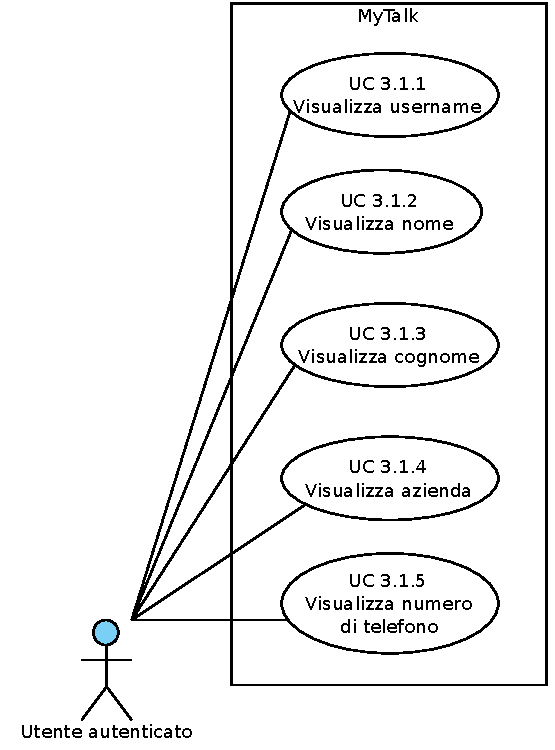
\includegraphics[scale=0.7]{./casi_uso/UC3-1.pdf}
\caption{UC 3.1 Visualizzazione dei dati dell'utente.}
\end{figure}

\noindent
\textbf{Attori primari:} utente autenticato.\\
\textbf{Descrizione:} l'utente visualizza i suoi dati.\\
\textbf{Precondizione:} l'utente vuole visualizzare i suoi dati.\\
\textbf{Postcondizione:} il sistema ha mostrato all'utente i dati che desiderava.\\
\textbf{Scenario principale:}
\begin{itemize}
\item l'utente visualizza i propri dati.
\end{itemize}

\subsubsection{UC 3.1.1 Visualizza username}
\noindent 
\textbf{Attori primari:} utente autenticato.\\
\textbf{Descrizione:} l'utente visualizza il suo username.\\
\textbf{Precondizione:} l'utente vuole visualizzare i propri dati.\\
\textbf{Postcondizione:} il sistema ha mostrato all'utente la propria username.\\
\textbf{Scenario principale:}
\begin{itemize}
\item l'utente visualizza il proprio username.
\end{itemize}

\subsubsection{UC 3.1.2 Visualizza nome}
\noindent 
\textbf{Attori primari:} utente autenticato.\\
\textbf{Descrizione:} l'utente visualizza il proprio nome.\\
\textbf{Precondizione:} l'utente vuole visualizzare i propri dati.\\
\textbf{Postcondizione:} il sistema ha mostrato all'utente il proprio nome.\\
\textbf{Scenario principale:}
\begin{itemize}
\item l'utente visualizza il proprio nome.
\end{itemize}

\subsubsection{UC 3.1.3 Visualizza cognome}
\noindent 
\textbf{Attori primari:} utente autenticato.\\
\textbf{Descrizione:} l'utente visualizza il suo cognome.\\
\textbf{Precondizione:} l'utente vuole visualizzare i propri dati.\\
\textbf{Postcondizione:} il sistema ha mostrato all'utente il proprio cognome.\\
\textbf{Scenario principale:}
\begin{itemize}
\item l'utente visualizza il proprio cognome.\\
\end{itemize}

\subsubsection{UC 3.1.4 Visualizza azienda}
\noindent 
\textbf{Attori primari:} utente autenticato.\\
\textbf{Descrizione:} l'utente visualizza il suo cognome.\\
\textbf{Precondizione:} l'utente vuole visualizzare i propri dati.\\
\textbf{Postcondizione:} il sistema ha mostrato all'utente il nome dell'azienda per cui lavora.\\
\textbf{Scenario principale:}
\begin{itemize}
\item l'utente visualizza il nome dell'azienda per cui lavora.\\
\end{itemize}

\subsubsection{UC 3.1.5 Visualizza numero di telefono}
\noindent 
\textbf{Attori primari:} utente autenticato.\\
\textbf{Descrizione:} l'utente visualizza il suo numero di telefono.\\
\textbf{Precondizione:} l'utente vuole visualizzare i propri dati.\\
\textbf{Postcondizione:} il sistema ha mostrato all'utente il proprio numero di telefono, il sistema ha terminato la visualizzazione dei dati.\\
\textbf{Scenario principale:}
\begin{itemize}
\item l'utente visualizza il proprio numero di telefono.\\
\end{itemize}

\newpage

\subsubsection{UC 3.2 Modifica dati utente}

\begin{figure}[htbp]
\centering
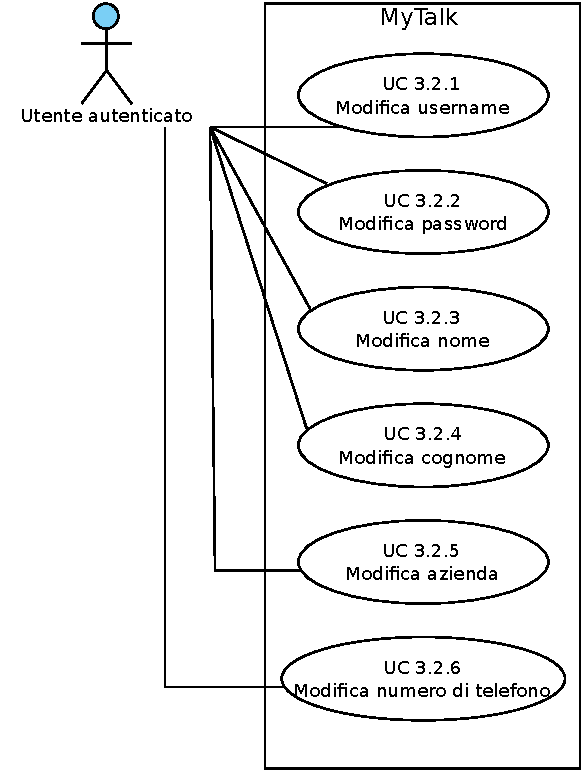
\includegraphics[scale=0.7]{./casi_uso/UC3-2.pdf}
\caption{UC 3.2 Modifica dei dati dell'utente.}
\end{figure}

\noindent
\textbf{Attori primari:} utente autenticato.\\
\textbf{Descrizione:} l'utente vuole modificare i propri dati; se i dati immessi dall'utente sono corretti il sistema registra i cambiamenti.\\
\textbf{Precondizione:} l'utente vuole modificare i suoi dati.\\
\textbf{Postcondizione:} il sistema ha salvato le modifiche dei dati dell'utente.\\
\textbf{Scenario principale:}
\begin{itemize}
\item l'utente sceglie quale dato modificare;
\item l'utente dopo aver scelto il dato da modificare, procede con il cambiamento;
\item il sistema cambia il dato con quello indicato dall'utente.
\end{itemize}

\subsubsection{UC 3.2.1 Modifica username}

\noindent
\textbf{Attori primari:} utente autenticato.\\
\textbf{Descrizione:} l'utente inserisce il proprio username, se lo username risulta non essere ancora utilizzato da un altro utente allora il cambiamento viene registrato nel sistema.\\
\textbf{Precondizione:} l'utente vuole modificare il suo username.\\
\textbf{Postcondizione:} il cambiamento di username viene salvato dal sistema.\\
\textbf{Scenario principale:}
\begin{itemize}
\item l'utente inserisce il nuovo username scelto.
\end{itemize}
\textbf{Scenario alternativo:} il nuovo username risulta essere già presente nel sistema, ne viene data comunicazione all'utente che può reinserire il dato.

\newpage

\subsubsection{UC 3.2.2 Modifica password}

\begin{figure}[htbp]
\centering
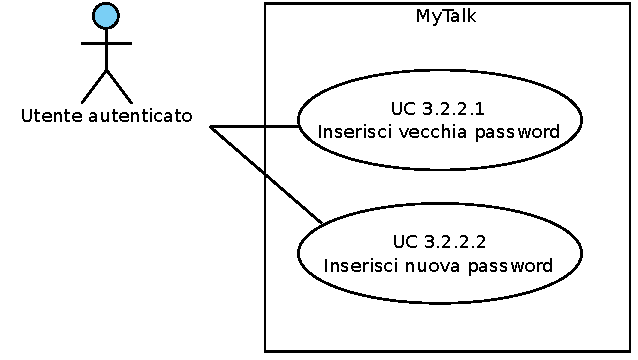
\includegraphics[scale=0.7]{./casi_uso/UC3-2-2.pdf}
\caption{UC 3.2.2 Modifica della password dell'utente.}
\end{figure}

\noindent
\textbf{Attori primari:} utente autenticato.\\
\textbf{Descrizione:} l'utente inserisce la vecchia password, la nuova password e la conferma della nuova password. Se la vecchia password corrisponde alla password corrente e la nuova password corrisponde alla sua conferma, allora i dati sono validi e il cambiamento viene registrato nel sistema.\\
\textbf{Precondizione:} l'utente vuole modificare la sua password.\\
\textbf{Postcondizione:} il sistema ha effettuato il cambio della password come richiesto dall'utente.\\
\textbf{Scenario principale:}
\begin{itemize}
\item l'utente inserisce la vecchia password;
\item l'utente inserisce la nuova password scelta;
\item l'utente inserisce la conferma della password.
\end{itemize}
\textbf{Scenario alternativo: }la password corrente non corrisponde alla vecchia password inserita, l'utente ne riceve comunicazione e può reinserire il dato.\\
\textbf{Scenario alternativo:} le due nuove password inserite (la nuova password e la sua conferma) risultano essere diverse, ne viene data comunicazione all'utente che può reinserire i dati.

\subsubsection{UC 3.2.2.1 Inserisci vecchia password}
\noindent
\textbf{Attori primari:} utente autenticato.\\
\textbf{Descrizione:} l'utente inserisce la vecchia password.\\
\textbf{Precondizione:} l'utente vuole modificare la sua password.\\
\textbf{Postcondizione:} la vecchia password è stata digitata.\\
\textbf{Scenario principale:}
\begin{itemize}
\item l'utente inserisce la sua vecchia password.
\end{itemize}

\subsubsection{UC 3.2.2.2 Inserisci nuova password}
\noindent
\textbf{Attori primari:} utente autenticato.\\
\textbf{Descrizione:} l'utente inserisce la nuova password scelta.\\
\textbf{Precondizione:} l'utente vuole modificare la sua password.\\
\textbf{Postcondizione:} la nuova password è stata digitata.\\
\textbf{Scenario principale:}
\begin{itemize}
\item l'utente inserisce la nuova password scelta.
\end{itemize}

\subsubsection{UC 3.2.3 Modifica nome}
\noindent
\textbf{Attori primari:} utente autenticato.\\
\textbf{Descrizione:} l'utente inserisce il nuovo nome, il sistema procede con il cambiamento del dato.\\
\textbf{Precondizione:} l'utente vuole modificare il suo nome salvato nel sistema.\\
\textbf{Postcondizione:} il cambiamento di nome viene salvato dal sistema.\\
\textbf{Scenario principale:}
\begin{itemize}
\item l'utente inserisce il nuovo nome scelto.
\end{itemize}

\subsubsection{UC 3.2.4 Modifica cognome}
\noindent
\textbf{Attori primari:} utente autenticato.\\
\textbf{Descrizione:} l'utente inserisce il nuovo cognome, il sistema procede con il cambiamento del dato.\\
\textbf{Precondizione:} l'utente vuole modificare il suo cognome salvato nel sistema.\\
\textbf{Postcondizione:} il cambiamento di cognome viene salvato dal sistema.\\
\textbf{Scenario principale:}
\begin{itemize}
\item l'utente inserisce il nuovo cognome scelto.
\end{itemize}

\subsubsection{UC 3.2.5 Modifica azienda}
\noindent
\textbf{Attori primari:} utente autenticato.\\
\textbf{Descrizione:} l'utente inserisce il nuovo nome dell'azienda che deve apparire come datrice di lavoro, il sistema procede con il cambiamento del dato.\\
\textbf{Precondizione:} l'utente vuole modificare il nome dell'azienda datrice di lavoro salvato nel sistema.\\
\textbf{Postcondizione:} il cambiamento di nome di azienda viene salvato dal sistema.\\
\textbf{Scenario principale:}
\begin{itemize}
\item l'utente inserisce il nuovo nome dell'azienda.
\end{itemize}

\subsubsection{UC 3.2.6 Modifica numero di telefono}
\noindent
\textbf{Attori primari:} utente autenticato.\\
\textbf{Descrizione:} l'utente inserisce il nuovo numero di telefono, il sistema procede con il cambiamento del dato.\\
\textbf{Precondizione:} l'utente vuole modificare il suo numero di telefono salvato nel sistema.\\
\textbf{Postcondizione:} il cambiamento di numero di telefono viene salvato dal sistema.\\
\textbf{Scenario principale:}
\begin{itemize}
\item l'utente inserisce il nuovo numero di telefono.
\end{itemize}

\newpage

\subsubsection{UC 4 Comunicazione audio e video}

\begin{figure}[htbp]
\centering
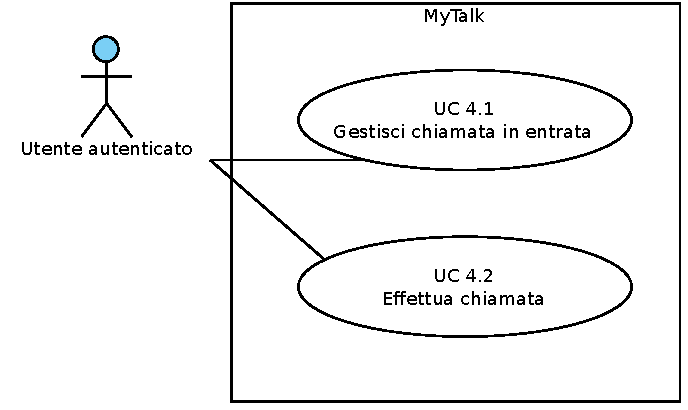
\includegraphics[scale=0.7]{./casi_uso/UC4.pdf}
\caption{UC 4 Comunicazione audio e video.}
\end{figure}

\noindent
\textbf{Attori primari: }utente autenticato.\\
\textbf{Descrizione: }l'utente è autenticato, al momento non ci sono chiamate attive e l'utente vuole o accettare una chiamata in arrivo o ne vuole effettuare una.\\
\textbf{Precondizione: }il sistema è funzionante e l'utente autenticato vuole comunicare accettando una chiamata in arrivo o effettuandone una. Al momento non ci sono chiamate attive.\\
\textbf{Postcondizione: }l'utente ha terminato la chiamata, il sistema dopo aver chiuso la comunicazione si trova nello stato immediatamente successivo al login (figura: \ref{figUC0}).\\
\textbf{Scenario principale:}
\begin{itemize}
\item l'utente può gestire chiamate in arrivo;
\item l'utente può effettuare chiamate.
\end{itemize}

\subsubsection{UC 4.1 Gestisci chiamata in entrata}

\begin{figure}[htbp]
\centering
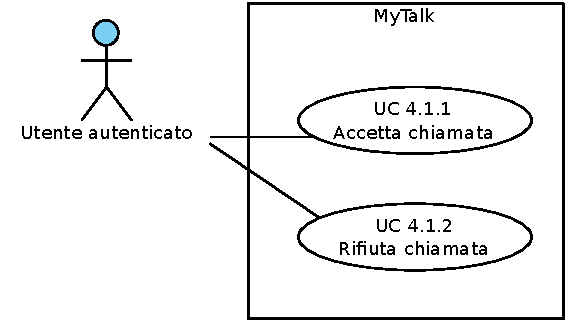
\includegraphics[scale=0.7]{./casi_uso/UC4-1.pdf}
\caption{UC 4.1 Gestione della chiamata in entrata.}
\end{figure}

\noindent
\textbf{Attori primari:} utente autenticato.\\
\textbf{Descrizione:} l'utente è autenticato, al momento non ci sono chiamate attive e viene data notifica di una chiamata in entrata.\\
\textbf{Precondizione:} il sistema è funzionante e l'utente autenticato sta ricevendo una chiamata in entrata.\\
\textbf{Postcondizione:} la chiamata è stata chiusa o rifiutata da parte dell'utente, il sistema si trova nello stato immediatamente successivo al login (figura: \ref{figUC0}) pronto ad effettuare nuove operazioni.\\
\textbf{Scenario principale:}
\begin{itemize}
\item l'utente riceve una chiamata;
\item l'utente può accettare la chiamata;
\item l'utente può rifiutare la chiamata.
\end{itemize}

\subsubsection{UC 4.1.1 Accetta chiamata}

\begin{figure}[htbp]
\centering
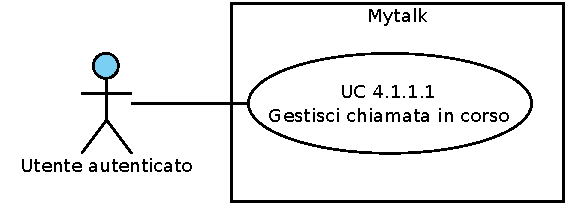
\includegraphics[scale=0.7]{./casi_uso/UC4-1-1.pdf}
\caption{UC 4.1.1 La chiamata in entrata viene accettata.}
\end{figure}

\noindent\textbf{Attori primari:} utente autenticato.\\
\textbf{Descrizione:} l'utente ha scelto di gestire una comunicazione in entrata e ha scelto di accettare la chiamata, deve quindi gestire la chiamata in corso eventualmente anche solo chiudendola.\\
\textbf{Precondizione:} l'utente è autenticato. Il sistema è funzionante, l'utente ha scelto di gestire una chiamata in arrivo accettandola.\\
\textbf{Postcondizione:} il sistema ha chiuso la chiamata.\\
\textbf{scenario principale:}
\begin{itemize}
\item la chiamata viene accettata;
\item l'utente può gestire la chiamata in corso.
\end{itemize}

\newpage

\subsubsection{UC 4.1.1.1 Gestisci chiamata in corso}
\label{sec:UC4-1-1-1GestioneChiamata}

\begin{figure}[htbp]
\centering
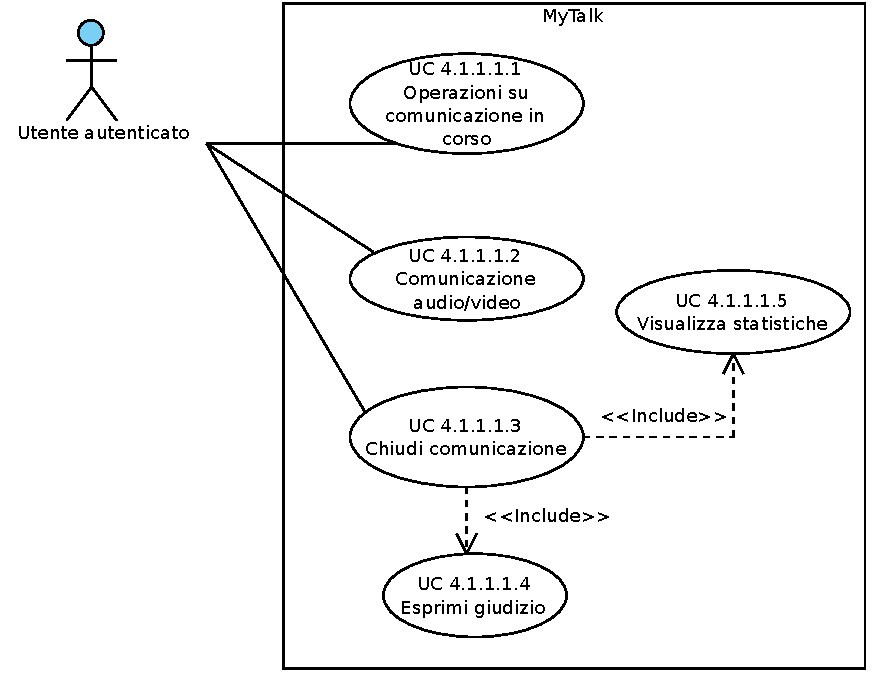
\includegraphics[scale=0.7]{./casi_uso/UC4-1-1-1.pdf}
\label{figUC4-1-1-1}
\caption{UC 4.1.1.1 Gestione della chiamata in corso.}
\end{figure}

\noindent\textbf{Attori primari:} utente autenticato.\\
\textbf{Descrizione:} una chiamata è appena iniziata, si possono quindi eseguire delle operazioni sulla comunicazione e successivamente chiuderla visualizzando statistiche sull'attività. Vi \`e l'opzione di esprimere un giudizio sulla qualità del servizio.\\
\textbf{Precondizione:} l'utente è autenticato. Il sistema è funzionante e una comunicazione è appena iniziata.\\
\textbf{Postcondizione:} il sistema chiude la chiamata su richiesta dell'utente, visualizzando le statistiche sull'uso e invitando l'utente ad esprimere un giudizio sulla qualità del servizio.\\
\textbf{Scenario principale:}
\begin{itemize}
\item la chiamata viene accettata;
\item gli utenti che partecipano alla chiamata si scambiano segnali audio e video (videochiamata);
\item possono venire effettuate delle operazioni durante la chiamata;
\item la chiamata viene chiusa, vengono visualizzate statistiche sull'attività e viene invitato l'utente ad esprimere un giudizio sul servizio fruito.
\end{itemize}

\newpage

\subsubsection{UC 4.1.1.1.1 Operazioni su comunicazione in corso}

\begin{figure}[htbp]
\centering
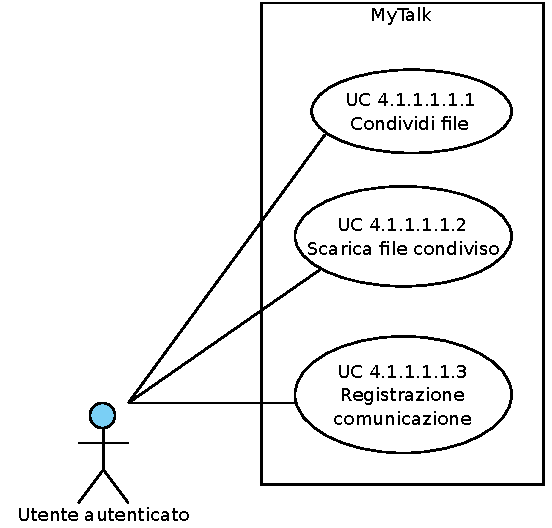
\includegraphics[scale=0.7]{./casi_uso/UC4-1-1-1-1.pdf}
\caption{UC 4.1.1.1.1 Operazioni che è possibile eseguire mentre la chiamata è in corso.}
\end{figure}

\noindent
\textbf{Attori primari:} utente autenticato.\\
\textbf{Descrizione:} una chiamata è in corso ed è possibile effettuare operazioni.\\
\textbf{Precondizione:} l'utente è autenticato. Il sistema è funzionante e una comunicazione è in atto.\\
\textbf{Postcondizione:} il sistema ha permesso agli utenti di operare sulla chiamata fino alla chiusura della comunicazione.\\
\textbf{Scenario principale:}
\begin{itemize}
\item la chiamata è in corso;
\item l'utente può condividere dati;
\item l'utente può registrare la chiamata;
\item l'utente può scaricare file condivisi da uno degli utenti partecipanti alla chiamata.
\end{itemize}

\subsubsection{UC 4.1.1.1.1.1 Condividi file}
\noindent
\textbf{Attori primari:} utente autenticato.\\
\textbf{Descrizione:} l'utente vuole condividere un file con l'utente o gli utenti che partecipano alla chiamata in corso.\\
\textbf{Precondizione:} l'utente è autenticato, il sistema è funzionante, una comunicazione è in atto e l'utente vuole condividere un file con gli altri utenti che partecipano alla chiamata.\\
\textbf{Postcondizione:} dopo la condivisione del file la chiamata continua e gli altri utenti possono scaricare il file condiviso.\\
\textbf{Scenario principale:}
\begin{itemize}
\item la chiamata è in corso;
\item l'utente condivide un file con gli altri utenti;
\item il file è scaricabile dagli altri utenti;
\end{itemize}

\subsubsection{UC 4.1.1.1.1.2 Scarica file condiviso}
\noindent
\textbf{Attori primari:} utente autenticato.\\
\textbf{Descrizione:} l'utente vuole scaricare un file precedentemente condiviso da un altro partecipante alla chiamata. Durante il download del file la chiamata continua normalmente.\\
\textbf{Precondizione:} l'utente è autenticato, il sistema è funzionante, una comunicazione è in atto e l'utente vuole scaricare un file precedentemente condiviso da un altro partecipante alla chiamata.\\
\textbf{Postcondizione:} dopo aver scaricato il file condiviso la chiamata continua.\\
\textbf{scenario principale:}
\begin{itemize}
\item la chiamata è in corso;
\item l'utente scarica un file condiviso da un altro partecipante;
\item la chiamata non viene interrotta durante questa operazione.
\end{itemize}

\subsubsection{UC 4.1.1.1.1.3 Registrazione comunicazione}
\noindent 
\textbf{Attori primari:} utente autenticato.\\
\textbf{Descrizione:} l'utente una volta che è stata instaurata una comunicazione audio/video può decidere di registrarla. Durante la registrazione la chiamata continua normalmente.\\
\textbf{Precondizione:} una comunicazione è in atto e l'utente decide di registrarne il contenuto su un file audio/video.\\
\textbf{Postcondizione:} la registrazione si conclude a causa o di una richiesta dell'utente o della fine della chiamata. La registrazione in ambo i casi è completata.\\
\textbf{Scenario principale:}
\begin{itemize}
\item una chiamata è in corso;
\item l'utente richiede la registrazione della chiamata;
\item la registrazione si avvia;
\item la registrazione si conclude a causa o di una richiesta dell'utente o a causa del termine della comunicazione;
\item la registrazione è completata e viene salvata.
\end{itemize}

\newpage

\subsubsection{UC 4.1.1.1.2 Comunicazione audio/video}

\begin{figure}[htbp]
\centering
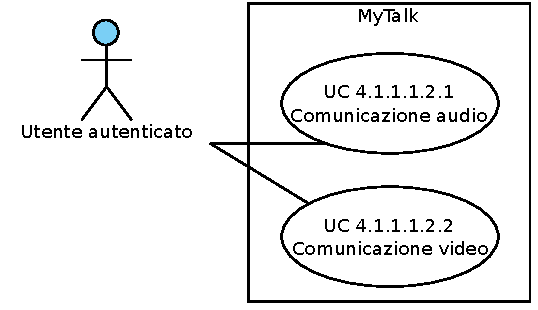
\includegraphics[scale=0.7]{./casi_uso/UC4-1-1-1-2.pdf}
\caption{UC 4.1.1.1.2 Scambio del segnale audio/video.}
\end{figure}

\noindent
\textbf{Attori primari:} utente autenticato.\\
\textbf{Descrizione:} una chiamata è in corso ed è possibile per gli utenti chiamare scambiandosi in tempo reale segnale audio/video.\\
\textbf{Precondizione:} l'utente è autenticato, il sistema è funzionante e una comunicazione è in atto.\\
\textbf{Postcondizione:} il sistema ha chiuso la chiamata.\\
\textbf{Scenario principale:}
\begin{itemize}
\item la chiamata è in corso;
\item è possibile per i partecipanti comunicare in tempo reale trasmettendo segnale audio e video;
\item il segnale viene interrotto quando la chiamata termina.
\end{itemize}
\textbf{Scenario alternativo:} è impossibile ricevere e/o inviare il segnale audio e/o video e quindi l'utente che ha tentato di effettuare la comunicazione viene avvisato in maniera opportuna e può eventualmente chiudere la comunicazione.

\subsubsection{UC 4.1.1.1.2.1 Comunicazione audio}
\noindent
\textbf{Attori primari:} utente autenticato.\\
\textbf{Descrizione:} una chiamata è in corso ed è possibile per gli utenti chiamare scambiandosi in tempo reale segnale audio.\\
\textbf{Precondizione:} l'utente è autenticato, il sistema è funzionante e una comunicazione è in atto.\\
\textbf{Postcondizione:} il sistema ha chiuso la chiamata.\\
\textbf{Scenario principale:}
\begin{itemize}
\item la chiamata è in corso;
\item è possibile per i partecipanti comunicare in tempo reale trasmettendo segnale audio;
\item il segnale viene interrotto quando la chiamata termina.
\end{itemize}
\textbf{Scenario alternativo:} è impossibile ricevere e/o inviare il segnale audio e quindi l'utente che ha tentato di effettuare la comunicazione viene avvisato in maniera opportuna e può eventualmente chiudere la comunicazione.

\subsubsection{UC 4.1.1.1.2.2 Comunicazione video}
\noindent
\textbf{Attori primari:} utente autenticato.\\
\textbf{Descrizione:} una chiamata è in corso ed è possibile per gli utenti chiamare scambiandosi in tempo reale segnale video.\\
\textbf{Precondizione:} l'utente è autenticato, il sistema è funzionante e una comunicazione è in atto.\\
\textbf{Postcondizione:} il sistema ha chiuso la chiamata.\\
\textbf{Scenario principale:}
\begin{itemize}
\item la chiamata è in corso;
\item è possibile per i partecipanti comunicare in tempo reale trasmettendo segnale video;
\item il segnale viene interrotto quando la chiamata termina.
\end{itemize}
\textbf{Scenario alternativo:} è impossibile ricevere e/o inviare il segnale video e quindi l'utente che ha tentato di effettuare la comunicazione viene avvisato in maniera opportuna e può eventualmente chiudere la comunicazione.

\subsubsection{UC 4.1.1.1.3 Chiudi comunicazione}
\noindent 
\textbf{Attori principali:} utente autenticato.\\
\textbf{Descrizione:} l'utente o richiede la chiusura della chiamata o riceve tale richiesta. Vengono quindi visualizzate le statistiche che poi verranno inviate (indipendentemente dalla volontà dell'utente) al server$_{|g|}$ per permettere il monitoraggio dell'applicazione. Inoltre viene chiesto all'utente un parere positivo o negativo sulla qualità della comunicazione. Anche tale parere verrà inviato al server$_{|g|}$ dell'applicazione.\\
\textbf{Precondizione:} viene o giunge richiesta di interruzione della comunicazione, una chiamata è in atto, il sistema è funzionante.\\
\textbf{Postcondizione:} la chiamata è stata chiusa e le statistiche assieme alla valutazione dell'utente sulla qualità della comunicazione sono state inviate al server. Il sistema è pronto a gestire altre comunicazioni (cap. \ref{sec:UC0generale}).\\
\textbf{Scenario principale:}
\begin{itemize}
\item giunge richiesta di chiusura della comunicazione;
\item la chiamata viene chiusa;
\item vengono visualizzate le statistiche sull'attività;
\item viene richiesta una valutazione sulla qualità del servizio all'utente;
\item le statistiche e la valutazione vengono inviate al server$_{|g|}$;
\end{itemize}

\subsubsection{UC 4.1.1.1.4 Esprimi giudizio}

\noindent 
\textbf{Attori principali:} utente autenticato.\\
\textbf{Descrizione:} alla fine della chiamata viene chiesto all'utente un giudizio complessivo sulla comunicazione e sul servizio.\\
\textbf{Precondizione:} una chiamata è appena terminata e viene richiesto all'utente un giudizio complessivo, il giudizio è inserito come un numero intero in una scala da 1 a 5.\\
\textbf{Postcondizione:} il giudizio è stato espresso.\\
\textbf{Scenario principale:}
\begin{itemize}
\item all'utente viene richiesto un giudizio complessivo sulla qualità del servizio;
\item l'utente dà un giudizio in una scala da uno a cinque;
\item il giudizio viene inviato dall'applicazione al server$_{|g|}$.
\end{itemize}
\textbf{Scenario alternativo:} l'utente si rifiuta di dare un giudizio alla chiamata, il sistema prosegue ugualmente con l'invio delle statistiche ignorando il giudizio dell'utente che è quindi opzionale.\\
\textbf{Scenario alternativo: } l'utente non inserisce un numero valido per l'espressione di un giudizio, il sistema informa l'utente sull'errore ed invita l'utente a reinserire il dato.

\subsubsection{UC 4.1.1.1.5 Visualizza statistiche}

\begin{figure}[htbp]
\centering
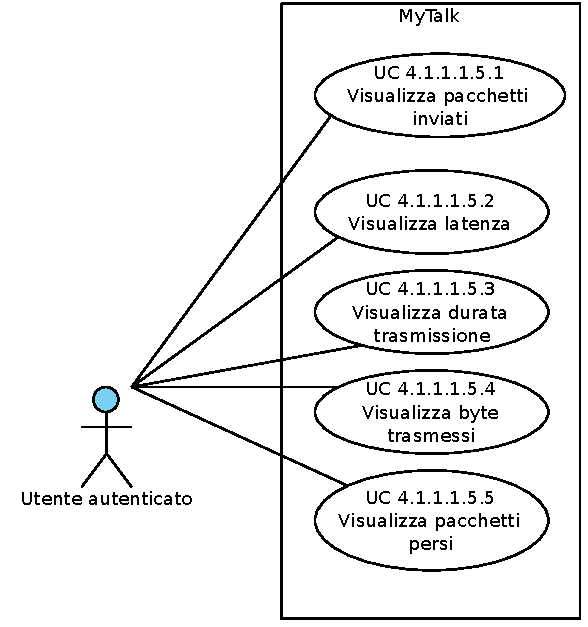
\includegraphics[scale=0.7]{./casi_uso/UC4-1-1-1-5.pdf}
\caption{UC 4.1.1.1.5 L'utente visualizza le statistiche sulla chiamata.}
\end{figure}

\noindent
\textbf{Attori primari:} utente autenticato.\\
\textbf{Descrizione:} l'utente una volta terminata la chiamata visualizza statistiche sull'attività: latenza$_{|g|}$, numero di pacchetti inviati, numero di pacchetti persi, quantità di byte scambiati, durata della comunicazione.\\
\textbf{Precondizione:} la chiamata è appena stata chiusa o dall'utente o dai partecipanti alla comunicazione.\\
\textbf{Postcondizione:} l'utente visualizza statistiche sull'attività.\\
\textbf{Scenario principale:}
\begin{itemize}
\item la chiamata viene chiusa;
\item l'utente visualizza statistiche sull'attività;
\end{itemize}

\subsubsection{UC 4.1.1.1.5.1 Visualizza pacchetti inviati}
\noindent
\textbf{Attori primari:} utente autenticato.\\
\textbf{Descrizione:} quando la chiamata viene chiusa, le statistiche vengono visualizzate e quindi anche il numero di pacchetti inviati.\\
\textbf{Precondizione:} l'utente ha chiuso la chiamata e visualizza le statistiche sull'attività.\\
\textbf{Postcondizione:} l'utente ha visualizzato il numero di pacchetti inviati.\\
\textbf{Scenario principale:}
\begin{itemize}
\item l'utente visualizza il numero di pacchetti inviati.
\end{itemize}

\subsubsection{UC 4.1.1.1.5.2 Visualizza latenza$_{|g|}$}
\noindent
\textbf{Attori primari:} utente autenticato.\\
\textbf{Descrizione:} quando la chiamata viene chiusa, le statistiche vengono visualizzate e quindi anche la latenza$_{|g|}$.\\
\textbf{Precondizione:} l'utente ha chiuso la chiamata e visualizza le statistiche sull'attività.\\
\textbf{Postcondizione:} l'utente ha visualizzato la latenza$_{|g|}$.\\
\textbf{Scenario principale:}
\begin{itemize}
\item l'utente visualizza la latenza$_{|g|}$.
\end{itemize}

\subsubsection{UC 4.1.1.1.5.3 Visualizza durata trasmissione}
\noindent
\textbf{Attori primari:} utente autenticato.\\
\textbf{Descrizione:} quando la chiamata viene chiusa, le statistiche vengono visualizzate e quindi anche la durata della comunicazione.\\
\textbf{Precondizione:} l'utente ha chiuso la chiamata e visualizza le statistiche sull'attività.\\
\textbf{Postcondizione:} l'utente ha visualizzato la durata della comunicazione.\\
\textbf{Scenario principale:}
\begin{itemize}
\item l'utente visualizza la durata della comunicazione.
\end{itemize}

\subsubsection{UC 4.1.1.1.5.4 Visualizza byte trasmessi}
\noindent 
\textbf{Attori principali:} utente autenticato.\\
\textbf{Descrizione:} alla fine della chiamata vengono visualizzati il numero totale di byte trasmessi.\\
\textbf{Precondizione:} una chiamata è appena terminata ed è stato possibile stimare il numero di byte trasmessi.\\
\textbf{Postcondizione:} i byte trasmessi sono stati visualizzati.\\
\textbf{Scenario principale:}
\begin{itemize}
\item l'utente visualizza il numero di byte trasmessi.
\end{itemize}

\subsubsection{UC 4.1.1.1.5.5 Visualizza pacchetti persi}
\noindent
\textbf{Attori primari:} utente autenticato.\\
\textbf{Descrizione:} quando la chiamata viene chiusa, le statistiche vengono visualizzate e quindi anche il numero di pacchetti persi.\\
\textbf{Precondizione:} l'utente ha chiuso la chiamata e visualizza le statistiche sull'attività.\\
\textbf{Postcondizione:} l'utente ha visualizzato il numero di pacchetti persi.\\
\textbf{Scenario principale:}
\begin{itemize}
\item l'utente visualizza il numero di pacchetti persi.
\end{itemize}

\subsubsection{UC 4.1.2 Rifiuta chiamata}
\noindent
\textbf{Attori primari:} utente autenticato.\\
\textbf{Descrizione:} una chiamata è in attesa, l'utente ricevente ha la facoltà di rifiutare la chiamata in entrata.\\
\textbf{Precondizione:} l'utente è autenticato, il sistema è funzionante e una chiamata è in attesa di accettazione.\\
\textbf{Postcondizione:} il sistema è nello stato immediatamente successivo al login (cap. \ref{sec:UC0generale}).\\
\textbf{Scenario principale:}
\begin{itemize}
\item la chiamata è in attesa;
\item la chiamata viene rifiutata;
\end{itemize}

\subsubsection{UC 4.2 Effettua chiamata}

\begin{figure}[htbp]
\centering
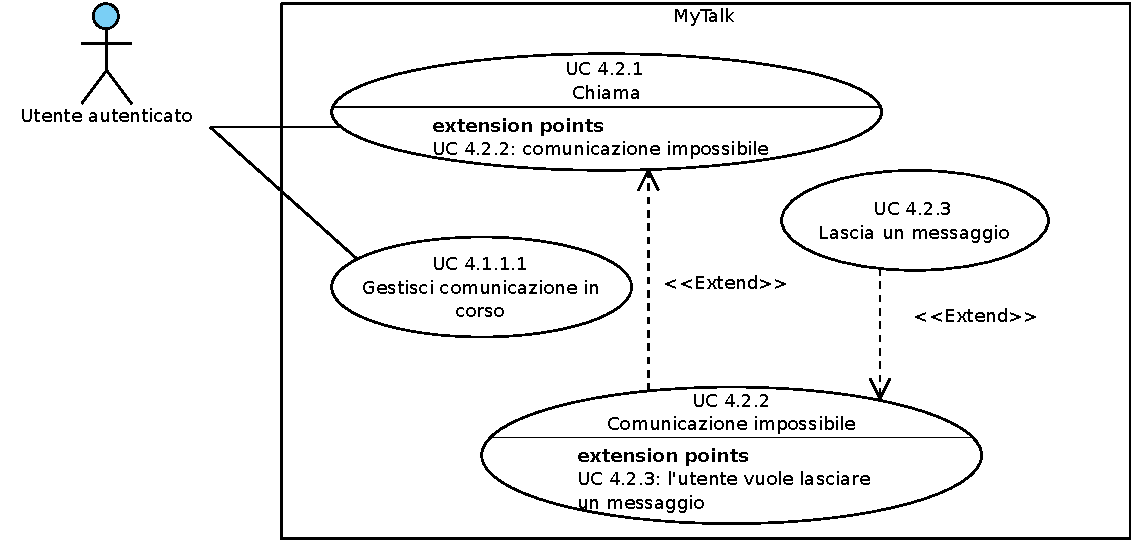
\includegraphics[scale=0.7]{./casi_uso/UC4-2.pdf}
\caption{UC 4.2 Procedura di effettuazione di una nuova chiamata.}
\end{figure}

\noindent
\textbf{Attori primari:} utente autenticato.\\
\textbf{Descrizione:} l'utente autenticato vuole effettuare una chiamata. Esso prima instaura la chiamata e dopo che questa è stata accettata dal ricevente, l'utente può gestire la comunicazione in corso. \\
\textbf{Precondizione:} l'utente è autenticato, il sistema è funzionante e l'utente autenticato vuole effettuare una chiamata.\\
\textbf{Postcondizione:} l'utente dopo aver effettuato e gestito la chiamata ha chiuso la comunicazione e il sistema si trova allo stato iniziale (figura: \ref{figUC0}), pronto ad effettuare nuove operazioni.\\
\textbf{Scenario principale:}
\begin{itemize}
\item l'utente autenticato può chiamare;
\item la chiamata viene accettata dal ricevente;
\item gli utenti partecipanti possono operare sulla comunicazione.
\end{itemize}

\newpage

\subsubsection{UC 4.2.1 Chiama}

\begin{figure}[htbp]
\centering
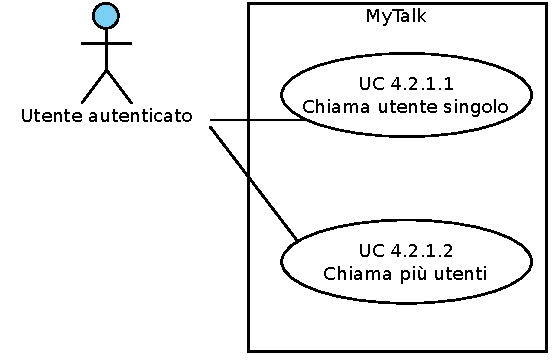
\includegraphics[scale=0.7]{./casi_uso/UC4-2-1.pdf}
\caption{UC 4.2.1 Procedura per effettuare una chiamata.}
\end{figure}

\noindent
\textbf{Attori primari:} utente autenticato.\\
\textbf{Descrizione:} l'utente autenticato vuole chiamare uno o più utenti registrati nel sistema. Qualora non sia possibile effettuare la chiamata l'utente ne riceve debita comunicazione e può registrare un messaggio (video o di testo) che poi l'utente ricevente visualizzerà in un secondo momento.\\
\textbf{Precondizione:} l'utente è autenticato, il sistema è funzionante e l'utente vuole chiamare uno o più utenti. Al momento non ci sono chiamate attive.\\
\textbf{Postcondizione:} la chiamata viene effettuata all'utente indicato, il sistema può gestire la chiamata in corso (figura: \ref{figUC4-1-1-1}) ma non può instaurare altre chiamate in contemporanea.\\
\textbf{Scenario principale:}
\begin{itemize}
\item l'utente può chiamare un solo utente;
\item l'utente può chiamare più di un utente.
\end{itemize}
\textbf{Scenario alternativo:} uno o più riceventi, indicati dall'utente che vuole effettuare la comunicazione, non si trovano all'interno del sistema. L'utente riceve debita comunicazione e può cambiare i dati immessi.\\
\textbf{Scenario alternativo:} la chiamata viene rifiutata o non è possibile effettuarla a causa di un malfunzionamento del sistema. L'utente ne riceve debita comunicazione e può scegliere di registrare un messaggio che verrà visualizzato in un secondo momento dai riceventi che non era stato possibile contattare. Il sistema, dopo aver registrato un eventuale messaggio, si ritrova allo stato immediatamente successivo al login (figura: \ref{figUC0}).

\newpage

\subsubsection{UC 4.2.1.1 Chiama utente singolo}

\begin{figure}[htbp]
\centering
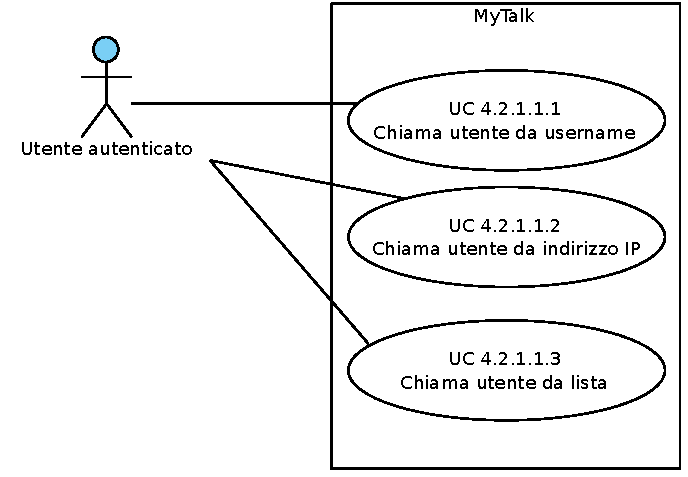
\includegraphics[scale=0.7]{./casi_uso/UC4-2-1-1.pdf}
\caption{UC 4.2.1.1 Procedura di effettuazione di una chiamata a un utente singolo.}
\end{figure}

\noindent
\textbf{Attori primari:} utente autenticato.\\
\textbf{Descrizione:} l'utente autenticato vuole contattare un altro utente registrato nel sistema, al momento non ci sono chiamate attive.\\
\textbf{Precondizione:} l'utente è autenticato, il sistema è funzionante e l'utente vuole chiamare un solo utente, non ci sono altre chiamate attive.\\
\textbf{Postcondizione:} la chiamata viene effettuata all'utente indicato tramite username o indirizzo IP o tramite la selezione dalla lista di utenti registrati al sistema, il sistema non può instaurare altre chiamate in contemporanea.\\
\textbf{Scenario principale:}
\begin{itemize}
\item l'utente può chiamare un utente di cui conosce lo username;
\item l'utente può chiamare un utente di cui conosce l'indirizzo IP$_{|g|}$;
\item l'utente può chiamare un utente selezionandolo tramite una lista.
\end{itemize}

\subsubsection{UC 4.2.1.1.1 Chiama utente da username}

\begin{figure}[htbp]
\centering
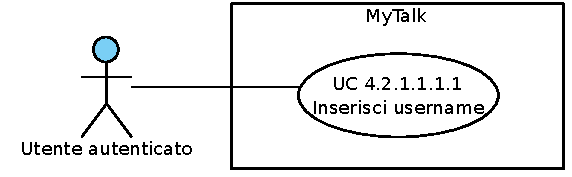
\includegraphics[scale=0.7]{./casi_uso/UC4-2-1-1-1.pdf}
\caption{UC 4.2.1.1.1 Chiamata di un singolo utente conoscendone lo username.}
\end{figure}

\noindent
\textbf{Attori primari:} utente autenticato.\\
\textbf{Descrizione:} l'utente autenticato vuole contattare un altro utente registrato nel sistema conoscendone lo username, inserisce quindi lo username e il sistema provvederà a chiamare l'utente ricevente.\\
\textbf{Precondizione:} l'utente è autenticato. Il sistema è funzionante e l'utente vuole chiamare un altro utente conoscendone lo username, non ci sono altre chiamate attive.\\
\textbf{Postcondizione:} la chiamata è stata effettuata dal sistema all'utente indicato tramite username, il sistema non può instaurare altre chiamate in contemporanea.\\
\textbf{Scenario principale:}
\begin{itemize}
\item l'utente inserisce lo username del ricevente;
\item il sistema dopo aver appurato che esiste un utente con lo username inserito chiama l'utente corrispondente.
\end{itemize}
\textbf{Scenario alternativo:} lo username inserito dall'utente non corrisponde ad alcun utente iscritto al sistema. All'utente ne viene data opportuna comunicazione dopodiché avrà la possibilità di ripetere l'operazione.

\subsubsection{UC 4.2.1.1.1.1 Inserisci username}
\noindent
\textbf{Attori primari:} utente autenticato.\\
\textbf{Descrizione:} l'utente autenticato vuole contattare un altro utente registrato nel sistema conoscendone lo username, quindi inserisce lo username.\\
\textbf{Precondizione:} l'utente è autenticato. Il sistema è funzionante e l'utente vuole chiamare un altro utente conoscendone lo username dunque lo inserisce.\\
\textbf{Postcondizione:} lo username è stato inserito, il sistema è pronto ad effettuare la chiamata.\\
\textbf{Scenario principale:}
\begin{itemize}
\item l'utente inserisce lo username del ricevente.
\end{itemize}

\subsubsection{UC 4.2.1.1.2 Chiama utente da indirizzo IP$_{|g|}$}

\begin{figure}[htbp]
\centering
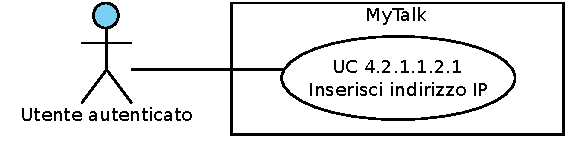
\includegraphics[scale=0.7]{./casi_uso/UC4-2-1-1-2.pdf}
\caption{UC4.2.1.1.2 Chiamata di un singolo utente conoscendone l'indirizzo IP$_{|g|}$.}
\end{figure}

\noindent
\textbf{Attori primari:} utente autenticato.\\
\textbf{Descrizione:} l'utente autenticato vuole contattare un altro utente registrato nel sistema conoscendone l'indirizzo IP$_{|g|}$. Inserisce quindi l'indirizzo IP$_{|g|}$ e il sistema provvederà a chiamare l'utente ricevente.\\
\textbf{Precondizione:} l'utente è autenticato. Il sistema è funzionante e l'utente vuole chiamare un altro utente tramite l'indirizzo IP$_{|g|}$, al momento non ci sono altre chiamate attive.\\
\textbf{Postcondizione:} la chiamata viene effettuata all'utente indicato tramite l'inserimento dell'indirizzo IP$_{|g|}$, il sistema non può instaurare altre chiamate in contemporanea.\\
\textbf{Scenario principale:}
\begin{itemize}
\item l'utente inserisce l'indirizzo IP$_{|g|}$ del ricevente;
\item il sistema dopo aver appurato che esiste un utente con quell'indirizzo IP$_{|g|}$ effettua la chiamata verso l'utente individuato.
\end{itemize}
\textbf{Scenario alternativo:} l'indirizzo IP$_{|g|}$ inserito non risulta appartenente ad alcun utente, il mittente viene avvisato del problema e può eventualmente reinserire il dato.

\subsubsection{UC 4.2.1.1.2.1 Inserisci indirizzo IP$_{|g|}$}
\noindent
\textbf{Attori primari:} utente autenticato.\\
\textbf{Descrizione:} l'utente autenticato vuole contattare un altro utente registrato nel sistema conoscendone l'indirizzo IP$_{|g|}$, inserisce quindi l'indirizzo IP$_{|g|}$.\\
\textbf{Precondizione:} l'utente è autenticato. Il sistema è funzionante e l'utente vuole chiamare un altro utente conoscendone l'indirizzo IP$_{|g|}$ dunque lo inserisce.\\
\textbf{Postcondizione:} l'indirizzo IP$_{|g|}$ è stato inserito.\\
\textbf{Scenario principale:}
\begin{itemize}
\item l'utente inserisce l'indirizzo IP$_{|g|}$ del ricevente.
\end{itemize}

\subsubsection{UC 4.2.1.1.3 Chiama utente da lista}

\begin{figure}[htbp]
\centering
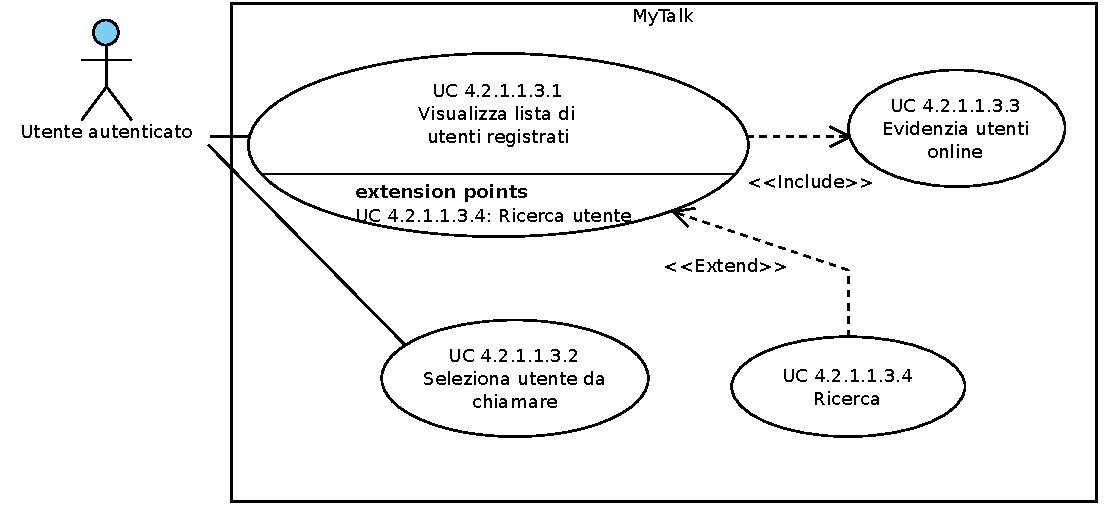
\includegraphics[scale=0.7]{./casi_uso/UC4-2-1-1-3.pdf}
\caption{UC 4.2.1.1.3 Chiamata di un singolo utente selezionandolo dalla lista degli utenti registrati.}
\end{figure}

\noindent
\textbf{Attori primari:} utente autenticato.\\
\textbf{Descrizione:} l'utente autenticato vuole contattare un altro utente selezionandolo dalla lista degli utenti registrati. L'utente visualizza la lista e sceglie l'utente che desidera chiamare.\\% eventualmente dopo averlo ricercato.\\
\textbf{Precondizione:} l'utente è autenticato. Il sistema è funzionante e l'utente vuole chiamare un utente selezionandolo dalla lista degli utenti registrati.\\
\textbf{Postcondizione:} il sistema effettua la chiamata all'utente indicato tramite la selezione tra gli utenti registrati al sistema, il sistema non può instaurare altre chiamate in contemporanea.\\
\textbf{Scenario principale:}
\begin{itemize}
\item l'utente visualizza la lista degli utenti registrati;
\item gli utenti online vengono evidenziati;
%\item l'utente può ricercare nella lista un utente;
\item l'utente seleziona l'utente che desidera chiamare;
\item l'utente selezionato viene chiamato.
\end{itemize}
\textbf{Scenario alternativo:} l'utente effettua una ricerca nella lista degli utenti registrati per trovare l'utente che vuole chiamare.

\subsubsection{UC 4.2.1.1.3.1 Visualizza lista di utenti registrati}
\noindent
\textbf{Attori primari:} utente autenticato.\\
\textbf{Descrizione:} l'utente autenticato vuole selezionare un utente dalla lista degli utenti registrati, che può visualizzare.\\ %Se lo richiede, in tale lista, può ricercare un utente sulla base dello username o sulla base dell'indirizzo IP$_{|g|}$ o sulla base del nome o sulla base del cognome o sulla base dell'azienda in cui lavora.\\
\textbf{Precondizione:} l'utente è autenticato, il sistema è funzionante e l'utente vuole selezionare un utente dalla lista degli utenti registrati.\\
\textbf{Postcondizione:} il sistema mostra all'utente la lista degli utenti registrati evidenziando quelli online e permettendo, su apposita richiesta da parte dell'utente la ricerca all'interno della lista.\\
\textbf{Scenario principale:}
\begin{itemize}
\item l'utente visualizza la lista degli utenti registrati al sistema;
\item gli utenti online vengono evidenziati;
%\item l'utente può ricercare in questa lista.
\end{itemize}
\textbf{Scenario alternativo:} l'utente effettua una ricerca nella lista degli utenti registrati per trovare l'utente che vuole chiamare. Può ricercare un utente sulla base dello username o sulla base dell'indirizzo IP$_{|g|}$ o sulla base del nome o sulla base del cognome o sulla base dell'azienda in cui lavora.

\subsubsection{UC 4.2.1.1.3.2 Seleziona utente da chiamare}
\noindent
\textbf{Attori primari:} utente autenticato.\\
\textbf{Descrizione:} viene visualizzata la lista degli utenti registrati. L'utente può cercare utenti nella lista e può selezionare un solo utente.\\
\textbf{Precondizione:} l'utente è autenticato. Il sistema è funzionante e l'utente vuole chiamare un altro utente selezionandolo dalla lista degli utenti registrati.\\
\textbf{Postcondizione:} l'utente ha selezionato un altro utente da chiamare dalla lista, il sistema effettua la chiamata all'utente selezionato, non sono possibili altre chiamate in contemporanea.\\
\textbf{Scenario principale:}
\begin{itemize}
\item l'utente seleziona l'utente che desidera chiamare, eventualmente dopo averlo ricercato;
\item l'utente scelto viene chiamato.
\end{itemize}

\subsubsection{UC 4.2.1.1.3.3 Evidenzia utenti online}
\noindent
\textbf{Attori primari:} utente autenticato.\\
\textbf{Descrizione:} l'utente visualizza la lista degli utenti registrati da selezionare per una eventuale chiamata e vengono evidenziati quelli online.\\
\textbf{Precondizione:} la lista correttamente visualizzata permette all'utente di scegliere il ricevente tra quelli registrati nel sistema.\\
\textbf{Postcondizione:} il sistema ha evidenziato gli utenti online come richiesto.\\
\textbf{Scenario principale:}
\begin{itemize}
\item gli utenti online vengono evidenziati all'interno della lista degli utenti registrati.
\end{itemize}

\newpage

\subsubsection{UC 4.2.1.1.3.4 Ricerca}

\begin{figure}[htbp]
\centering
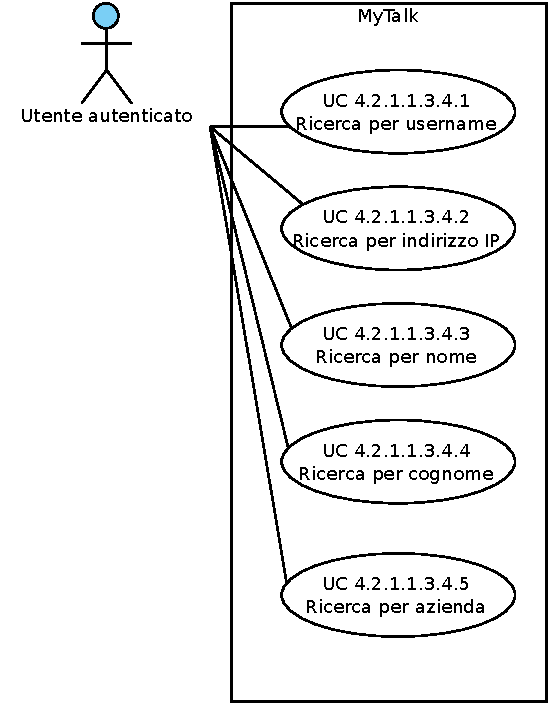
\includegraphics[scale=0.7]{./casi_uso/UC4-2-1-1-3-4.pdf}
\caption{UC 4.2.1.1.3.4 Ricerca di un utente all'interno della lista degli utenti registrati.}
\end{figure}

\noindent
\textbf{Attori primari:} utente autenticato.\\
\textbf{Descrizione:} l'utente può cercare un utente presente nella lista senza doverla scorrere indicandone lo username o l'indirizzo IP$_{|g|}$ o il nome o il cognome o l'azienda in cui lavora.\\
\textbf{Precondizione:} l'utente vuole cercare un utente nella lista senza scorrerla.\\
\textbf{Postcondizione:} il sistema ha visualizzato i risultati della ricerca.\\
\textbf{Scenario principale:}
\begin{itemize}
\item l'utente inserisce lo username o l'indirizzo IP$_{|g|}$ o il nome o il cognome o l'azienda dell'utente cercato;
\item l'utente visualizza nella lista i risultati della ricerca e può selezionare l'utente trovato.
\end{itemize}
\textbf{Scenario alternativo:} nessun utente viene trovato, quindi l'utente che ha effettuato la ricerca riceve debita comunicazione e può ripeterla.

\subsubsection{UC 4.2.1.1.3.4.1 Ricerca per username}
\noindent
\textbf{Attori primari:} utente autenticato.\\
\textbf{Descrizione:} l'utente cerca un utente presente nella lista senza doverla scorrere indicandone lo username.\\
\textbf{Precondizione:} l'utente vuole cercare un utente nella lista degli utenti registrati.\\
\textbf{Postcondizione:} il sistema ha mostrato i risultati della ricerca.\\
\textbf{Scenario principale:}
\begin{itemize}
\item l'utente inserisce lo username dell'utente cercato;
\item l'utente visualizza il risultato della ricerca.
\end{itemize}
\textbf{Scenario alternativo:} nessun utente viene trovato, quindi l'utente che ha effettuato la ricerca riceve debita comunicazione e può ripetere la ricerca.

\subsubsection{UC 4.2.1.1.3.4.2 Ricerca per indirizzo IP$_{|g|}$}
\noindent
\textbf{Attori primari:} utente autenticato.\\
\textbf{Descrizione:} l'utente cerca un utente presente nella lista, senza così doverla scorrere, indicandone l'indirizzo IP$_{|g|}$.\\
\textbf{Precondizione:} l'utente vuole cercare un utente nella lista senza scorrerla.\\
\textbf{Postcondizione:} il sistema ha mostrato i risultati della ricerca.\\
\textbf{Scenario principale:}
\begin{itemize}
\item l'utente inserisce l'indirizzo IP$_{|g|}$ dell'utente cercato;
\item l'utente visualizza il risultato della ricerca.
\end{itemize}
\textbf{Scenario alternativo:} nessun utente viene trovato, l'utente che ha effettuato la ricerca riceve debita comunicazione e può ripetere la ricerca.

\subsubsection{UC 4.2.1.1.3.4.3 Ricerca per nome}
\noindent
\textbf{Attori primari:} utente autenticato.\\
\textbf{Descrizione:} l'utente cerca un utente presente nella lista, senza così doverla scorrere, indicandone il nome.\\
\textbf{Precondizione:} l'utente vuole cercare un utente nella lista senza scorrerla.\\
\textbf{Postcondizione:} il sistema ha mostrato i risultati della ricerca.\\
\textbf{Scenario principale:}
\begin{itemize}
\item l'utente inserisce il nome dell'utente cercato;
\item l'utente visualizza il risultato della ricerca.
\end{itemize}
\textbf{Scenario alternativo:} nessun utente viene trovato, l'utente che ha effettuato la ricerca riceve debita comunicazione e può ripetere la ricerca.

\subsubsection{UC 4.2.1.1.3.4.4 Ricerca per cognome}
\noindent
\textbf{Attori primari:} utente autenticato.\\
\textbf{Descrizione:} l'utente cerca un utente presente nella lista, senza così doverla scorrere, indicandone il cognome.\\
\textbf{Precondizione:} l'utente vuole cercare un utente nella lista senza scorrerla.\\
\textbf{Postcondizione:} il sistema ha mostrato i risultati della ricerca.\\
\textbf{Scenario principale:}
\begin{itemize}
\item l'utente inserisce il cognome dell'utente cercato;
\item l'utente visualizza il risultato della ricerca.
\end{itemize}
\textbf{Scenario alternativo:} nessun utente viene trovato, l'utente che ha effettuato la ricerca riceve debita comunicazione e può ripetere la ricerca.

\subsubsection{UC 4.2.1.1.3.4.5 Ricerca per azienda}
\noindent
\textbf{Attori primari:} utente autenticato.\\
\textbf{Descrizione:} l'utente cerca un utente presente nella lista, senza così doverla scorrere, indicandone l'azienda di appartenenza.\\
\textbf{Precondizione:} l'utente vuole cercare un utente nella lista senza scorrerla.\\
\textbf{Postcondizione:} il sistema ha mostrato i risultati della ricerca.\\
\textbf{Scenario principale:}
\begin{itemize}
\item l'utente inserisce il nome dell'azienda di appartenenza dell'utente cercato;
\item l'utente visualizza il risultato della ricerca.
\end{itemize}
\textbf{Scenario alternativo:} nessun utente viene trovato, l'utente che ha effettuato la ricerca riceve debita comunicazione e può ripetere la ricerca.

\subsubsection{UC 4.2.1.2 Chiama più utenti}

\begin{figure}[htbp]
\centering
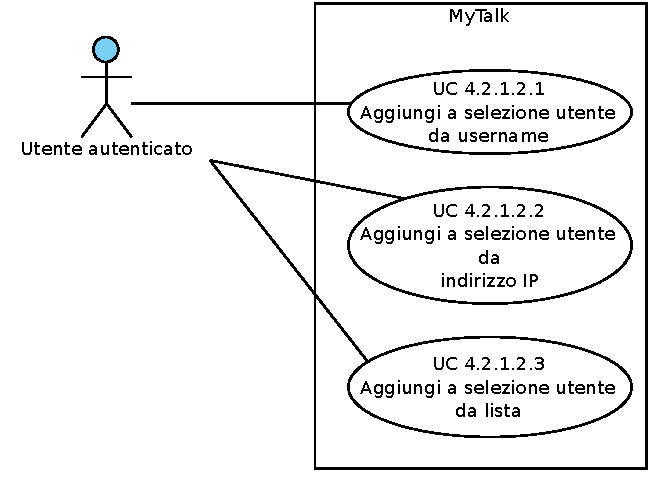
\includegraphics[scale=0.7]{./casi_uso/UC4-2-1-2.pdf}
\caption{UC 4.2.1.2 Procedura di effettuazione di una chiamata a più utenti.}
\end{figure}

\noindent
\textbf{Attori primari:} utente autenticato.\\
\textbf{Descrizione:} l'utente autenticato vuole contattare più utenti registrati al sistema.\\
\textbf{Precondizione:} l'utente è autenticato. Il sistema è funzionante e l'utente vuole chiamare più di un utente.\\
\textbf{Postcondizione:} il sistema effettua la chiamata agli utenti selezionati.\\
\textbf{Scenario principale:}
\begin{itemize}
\item l'utente può aggiungere alla selezione utenti di cui conosce lo username;
\item l'utente può aggiungere alla selezione utenti di cui conosce l'indirizzo IP$_{|g|}$;
\item l'utente può aggiungere alla selezione utenti selezionati dalla lista degli iscritti al server$_{|g|}$;
\end{itemize}

\newpage

\subsubsection{UC 4.2.1.2.1 Aggiungi a selezione utente da username}

\begin{figure}[htbp]
\centering
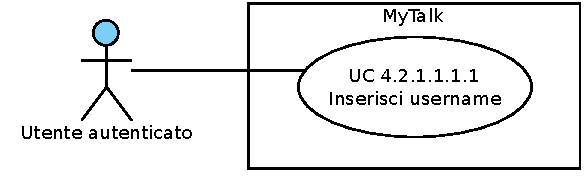
\includegraphics[scale=0.7]{./casi_uso/UC4-2-1-2-1.pdf}
\caption{UC 4.2.1.2.1 Aggiungi alla selezione un  utente tramite username.}
\end{figure}

\noindent
\textbf{Attori primari:} utente autenticato.\\
\textbf{Descrizione:} l'utente autenticato vuole aggiungere alla selezione degli utenti da chiamare un utente registrato al sistema conoscendone lo username. Esso inserisce quindi lo username e il sistema provvederà ad aggiungere l'utente corrispondente alla lista degli utenti che verranno chiamati.\\
\textbf{Precondizione:} l'utente è autenticato, il sistema è funzionante, l'utente vuole chiamare più utenti, l'utente vuole aggiungere alla selezione un utente conoscendone lo username.\\
\textbf{Postcondizione:} il sistema aggiunge l'utente a cui corrisponde lo username inserito alla lista degli utenti che verranno poi chiamati in videoconferenza.\\
\textbf{Scenario principale:}
\begin{itemize}
\item l'utente inserisce lo username del ricevente;
\item il sistema dopo aver appurato che esiste un utente con lo username inserito aggiunge l'utente corrispondente alla selezione degli utenti da chiamare.
\end{itemize}
\textbf{Scenario alternativo:} lo username inserito non corrisponde ad alcun utente iscritto al sistema. L'utente verrà avvisato del fallimento e potrà ripetere l'operazione.

\subsubsection{UC 4.2.1.2.2 Aggiungi a selezione utente da indirizzo IP$_{|g|}$}

\begin{figure}[htbp]
\centering
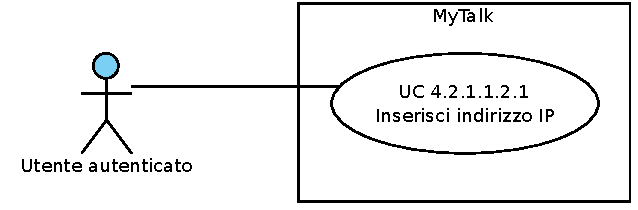
\includegraphics[scale=0.7]{./casi_uso/UC4-2-1-2-2.pdf}
\caption{UC 4.2.1.2.2 Aggiungi alla selezione un utente tramite indirizzo IP$_{|g|}$.}
\end{figure}

\noindent\textbf{Attori primari:} utente autenticato.\\
\textbf{Descrizione:} l'utente autenticato vuole aggiungere alla selezione degli utenti da chiamare un utente registrato al sistema conoscendone l'indirizzo IP$_{|g|}$. Esso inserisce quindi l'indirizzo IP$_{|g|}$ e il sistema provvederà ad aggiungere l'utente corrispondente alla lista degli utenti che verranno chiamati.\\
\textbf{Precondizione:} l'utente è autenticato, il sistema è funzionante, l'utente vuole chiamare più utenti, l'utente vuole aggiungere alla selezione un utente conoscendone l'indirizzo IP$_{|g|}$.\\
\textbf{Postcondizione:} il sistema aggiunge l'utente a cui corrisponde l'indirizzo IP$_{|g|}$ inserito alla lista degli utenti che verranno chiamati.\\
\textbf{Scenario principale:}
\begin{itemize}
\item l'utente inserisce l'indirizzo IP$_{|g|}$ del ricevente;
\item il sistema dopo aver appurato che esiste un utente con l'indirizzo IP$_{|g|}$ inserito aggiunge l'utente corrispondente alla selezione degli utenti da chiamare.
\end{itemize}
\textbf{Scenario alternativo:} l'indirizzo IP$_{|g|}$ inserito non corrisponde ad alcun utente iscritto al sistema. L'utente verrà avvisato del fallimento e potrà ripetere l'operazione.

\subsubsection{UC 4.2.1.2.3 Aggiungi a selezione utente da lista}

\begin{figure}[htbp]
\centering
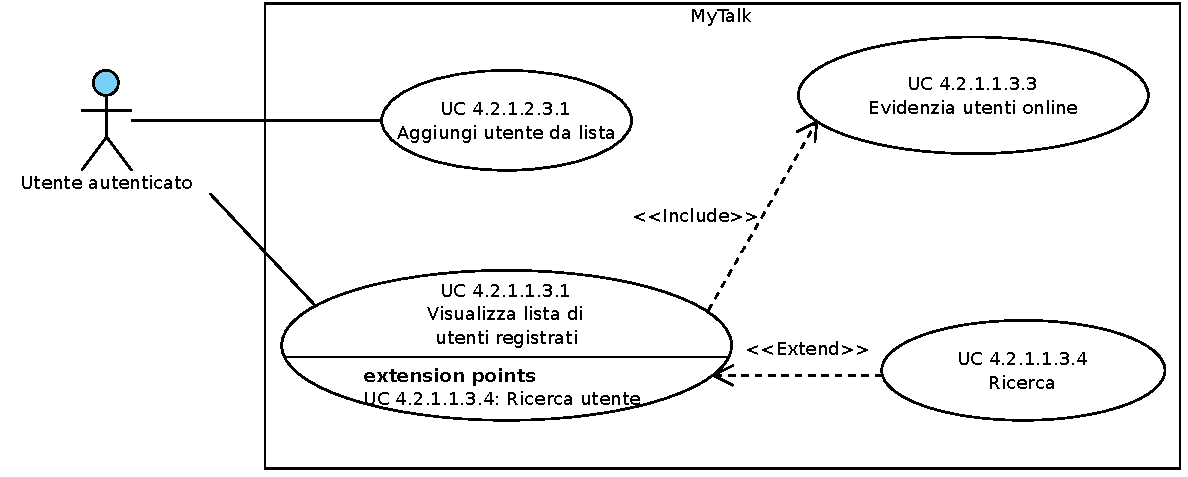
\includegraphics[scale=0.7]{./casi_uso/UC4-2-1-2-3.pdf}
\caption{UC 4.2.1.2.3 Aggiungi alla selezione un utente tramite lista.}
\end{figure}

\noindent
\textbf{Attori primari:} utente autenticato.\\
\textbf{Descrizione:} l'utente autenticato vuole contattare un altro utente selezionandolo dalla lista degli utenti registrati. L'utente può quindi visualizzare tale lista e scegliere l'utente che desidera aggiungere alla selezione.\\
\textbf{Precondizione:} l'utente è autenticato, il sistema è funzionante, l'utente vuole chiamare più utenti e vuole selezionarne almeno uno dalla lista di quelli registrati.\\
\textbf{Postcondizione:} il sistema aggiunge l'utente selezionato alla lista degli utenti che verranno poi chiamati in videoconferenza.\\
\textbf{Scenario principale:}
\begin{itemize}
\item l'utente visualizza la lista degli utenti registrati;
%\item l'utente può ricercare nella lista;
\item l'utente seleziona gli utenti che desidera aggiungere alla lista di quelli che verranno chiamati;
\item gli utenti selezionati sono stati aggiunti alla lista che verrà chiamata.
\end{itemize}
\textbf{Scenario alternativo:} l'utente effettua una ricerca nella lista degli utenti registrati per trovare l'utente che vuole chiamare.

\subsubsection{UC 4.2.1.2.3.1 Aggiungi utente da lista}
\noindent
\textbf{Attori primari:} utente autenticato.\\
\textbf{Descrizione:} viene visualizzata la lista degli utenti registrati. L'utente può cercarli in essa e può selezionare più di un utente da aggiungere alla lista che poi verrà chiamata.\\
\textbf{Precondizione:} l'utente è autenticato. Esso vuole chiamare più di un utente e vuole selezionarne almeno uno dalla lista degli utenti registrati.\\
\textbf{Postcondizione:} il sistema ha aggiunto gli utenti (possibilmente anche uno solo) alla lista degli utenti che poi verranno chiamati in videoconferenza.\\
\textbf{Scenario principale:}
\begin{itemize}
\item l'utente visualizza la lista degli utenti registrati;
\item gli utenti online vengono evidenziati;
\item l'utente può ricercare in questa lista;
\item l'utente seleziona uno o più utenti da aggiungere alla lista di quelli da chiamare;
\item gli utenti vengono aggiunti alla lista.
\end{itemize}

\subsubsection{UC 4.2.2 Comunicazione impossibile}
\noindent
\textbf{Attori primari:} utente autenticato.\\
\textbf{Descrizione:} l'utente autenticato vuole effettuare una chiamata ad uno o più utenti, chiama gli utenti, ma una o più persone rifiutano la comunicazione, oppure la comunicazione non è possibile per cause derivanti dal sistema (\emph{es}. assenza di connessione al server$_{|g|}$). In questo caso l'utente chiamante ha la possibilità di registrare un messaggio da recapitare poi agli utenti con cui desiderava comunicare.\\
\textbf{Precondizione:} l'utente è autenticato, il sistema è funzionante e l'utente autenticato vuole effettuare una chiamata, ha chiamato il destinatario ma la comunicazione per qualche motivo è impossibile.\\
\textbf{Postcondizione:} l'utente autenticato ha chiuso la comunicazione e il sistema è al punto immediatamente successivo al login (cap. \ref{sec:UC0generale}).\\
\textbf{Scenario principale:}
\begin{itemize}
\item la chiamata viene rifiutata o è impossibile instaurarla;
\item viene proposto all'utente di registrare un messaggio da visualizzare successivamente;
\item la comunicazione viene terminata.
\end{itemize}
\textbf{Scenario alternativo: }l'utente che ha effettuato la chiamata vuole registrare un messaggio. Il messaggio viene registrato e sarà visualizzato dal ricevente in un secondo momento.

\newpage

\subsubsection{UC 4.2.3 Lascia un messaggio }

\begin{figure}[htbp]
\centering
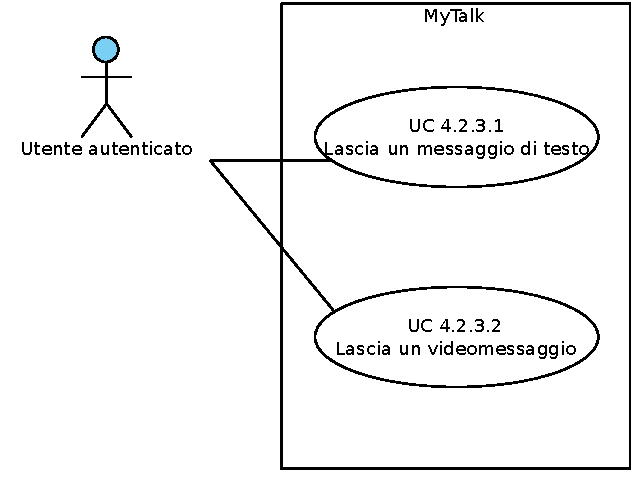
\includegraphics[scale=0.7]{./casi_uso/UC4-2-3.pdf}
\caption{UC 4.2.3 Lascia un messaggio.}
\end{figure}

\noindent
\textbf{Attori primari:} utente autenticato.\\
\textbf{Descrizione:} la chiamata da parte dell'utente è stata rifiutata o è impossibile comunicare per motivi non dipendenti dagli utenti e il mittente vuole lasciare un messaggio che poi il ricevente visualizzerà in un secondo momento.\\
\textbf{Precondizione:} l'ultima chiamata non è andata a buon fine, l'utente vuole lasciare un messaggio.\\
\textbf{Postcondizione:} l'utente ha lasciato un messaggio che il ricevente visualizzerà in un secondo momento.\\
\textbf{Scenario principale:}
\begin{itemize}
\item l'utente registra un messaggio per il ricevente, tale messaggio può essere o un messaggio di testo o un video messaggio.
\end{itemize}

\subsubsection{UC 4.2.3.1 Lascia un messaggio di testo}

\begin{figure}[htbp]
\centering
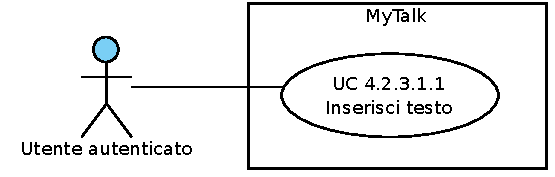
\includegraphics[scale=0.7]{./casi_uso/UC4-2-3-1.pdf}
\caption{UC 4.2.3.1 Lascia un messaggio di testo.}
\end{figure}

\noindent
\textbf{Attori primari:} utente autenticato.\\
\textbf{Descrizione:} la chiamata da parte dell'utente è stata rifiutata o è impossibile comunicare per motivi non dipendenti dagli utenti e il mittente vuole lasciare un messaggio testuale che poi il ricevente visualizzerà in un secondo momento.\\
\textbf{Precondizione:} l'ultima chiamata non è andata a buon fine, l'utente vuole lasciare un messaggio di testo.\\
\textbf{Postcondizione:} l'utente ha lasciato un messaggio testuale che il ricevente visualizzerà in un secondo momento.\\
\textbf{Scenario principale:}
\begin{itemize}
\item l'utente scrive un messaggio che poi l'utente ricevente visualizzerà.
\end{itemize}

\subsubsection{UC 4.2.3.1.1 Inserisci testo}
\noindent
\textbf{Attori primari:} utente autenticato.\\
\textbf{Descrizione:} l'ultima chiamata non è andata a buon fine, l'utente autenticato che effettua la chiamata inserisce il testo del messaggio che vuole lasciare all'utente chiamato.\\
\textbf{Precondizione:} l'ultima chiamata non è andata a buon fine, l'utente vuole inserire il testo del messaggio da lasciare all'utente chiamato.\\
\textbf{Postcondizione:} l'utente ha inserito il testo del messaggio che il ricevente visualizzerà in un secondo momento.\\
\textbf{Scenario principale:}
\begin{itemize}
\item l'utente inserisce il testo del messaggio che poi l'utente ricevente visualizzerà.
\end{itemize}

\subsubsection{UC 4.2.3.2 Lascia un video messaggio }

\begin{figure}[htbp]
\centering
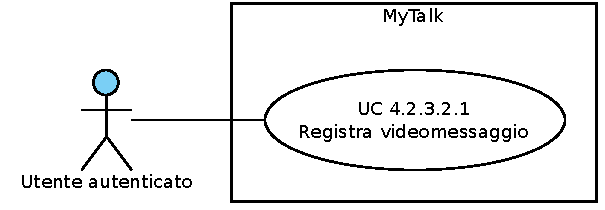
\includegraphics[scale=0.7]{./casi_uso/UC4-2-3-2.pdf}
\caption{UC 4.2.3.2 Lascia un video messaggio.}
\end{figure}

\noindent
\textbf{Attori primari:} utente autenticato.\\
\textbf{Descrizione:} la chiamata da parte dell'utente è stata rifiutata o è impossibile comunicare per motivi non dipendenti dagli utenti e il mittente vuole lasciare un video messaggio che poi il ricevente visualizzerà in un secondo momento.\\
\textbf{Precondizione:} l'ultima chiamata non è andata a buon fine, l'utente vuole lasciare un video messaggio.\\
\textbf{Postcondizione:} l'utente ha lasciato un video messaggio che il ricevente visualizzerà in un secondo momento.\\
\textbf{Scenario principale:}
\begin{itemize}
\item l'utente registra un video messaggio per il ricevente.
\end{itemize}

\subsubsection{UC 4.2.3.2.1 Registra video messaggio}
\noindent
\textbf{Attori primari:} utente autenticato.\\
\textbf{Descrizione:} l'ultima chiamata non è andata a buon fine, l'utente autenticato che effettua la chiamata registra il video messaggio che vuole lasciare all'utente chiamato.\\
\textbf{Precondizione:} l'ultima chiamata non è andata a buon fine, l'utente vuole registrare un video messaggio da lasciare all'utente chiamato.\\
\textbf{Postcondizione:} l'utente ha registrato il video messaggio che il ricevente visualizzerà in un secondo momento.\\
\textbf{Scenario principale:}
\begin{itemize}
\item l'utente registra il video messaggio che poi l'utente ricevente visualizzerà.
\end{itemize}

\newpage

\subsubsection{UC 5 Comunicazione chat}

\begin{figure}[htbp]
\centering
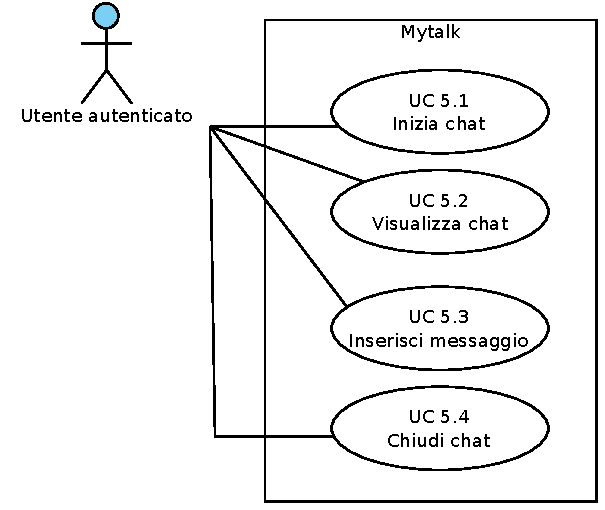
\includegraphics[scale=0.7]{./casi_uso/UC5.pdf}
\caption{UC 5 Comunicazione chat.}
\end{figure}

\noindent
\textbf{Attori primari:} utente autenticato.\\
\textbf{Descrizione:} l'utente vuole comunicare via chat con altri utenti (possibilmente uno solo), quindi può scrivere su una chat già esistente o può crearne una nuova selezionando gli utenti che vuole che partecipino alla chat. Non è possibile aggiungere altri utenti alla stessa chat una volta iniziata la comunicazione.\\
\textbf{Precondizione:} l'utente vuole comunicare tramite chat, è possibile che ci siano altre chat già aperte ed è possibile per l'utente poter chiamare durante l'esecuzione della chat.\\
\textbf{Postcondizione:} il sistema su richiesta dell'utente ha chiuso la chat.\\
\textbf{Scenario principale:}
\begin{itemize}
\item l'utente inizia una nuova chat o invitando altri utenti in chat o essendo invitato da altri utenti in chat;
\item l'utente può visualizzare la chat;
\item l'utente può scrivere sulla chat;
\item l'utente può abbandonare la chat, che rimane tuttavia attiva per gli altri utenti.
\end{itemize}

\newpage

\subsubsection{UC 5.1 Inizia chat}

\begin{figure}[htbp]
\centering
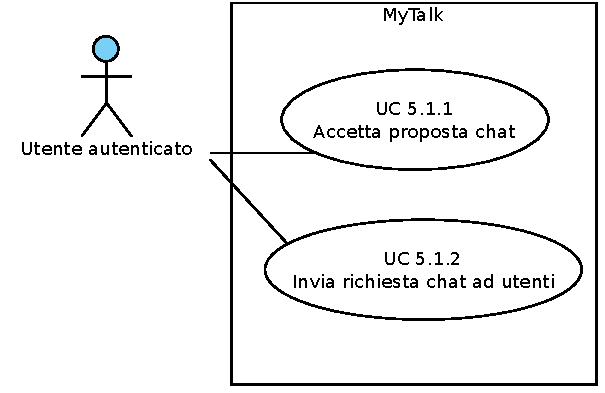
\includegraphics[scale=0.7]{./casi_uso/UC5-1.pdf}
\caption{UC 5.1 Inizia comunicazione chat.}
\end{figure}

\noindent
\textbf{Attori primari:} utente autenticato.\\
\textbf{Descrizione:} l'utente vuole iniziare a comunicare via chat con degli altri utenti, può quindi creare una nuova chat selezionando gli utenti che ne faranno parte.\\
\textbf{Precondizione:} l'utente vuole iniziare una nuova chat, è possibile che ci siano altre chat attive che coinvolgano l'utente che rimangono comunque attive.\\
\textbf{Postcondizione:} il sistema ha visualizzato una chat a cui l'utente fa parte.\\
\textbf{Scenario principale:}
\begin{itemize}
\item il sistema può aprire una chat a cui l'utente fa parte, accettando in modo automatico la richiesta di un altro utente;
\item l'utente può richiedere al sistema di creare una nuova chat alla quale faranno parte gli utenti indicati dall'utente che ha creato la chat.
\end{itemize}

\subsubsection{UC 5.1.1 Accetta proposta chat}
\noindent
\textbf{Attori primari:} utente autenticato.\\
\textbf{Descrizione:} l'utente riceve una proposta di chat, da parte di un altro utente. Il sistema apre una nuova chat in modo automatico.\\
\textbf{Precondizione:} l'utente ha ricevuto una proposta di chat.\\
\textbf{Postcondizione:} il sistema ha aperto una nuova chat.\\
\textbf{Scenario principale:}
\begin{itemize}
\item l'utente riceve una proposta di chat;
\item il sistema accetta in modo automatico la proposta ed apre una nuova chat.
\end{itemize}

\newpage

\subsubsection{UC 5.1.2 Invia richiesta chat ad utenti}

\begin{figure}[htbp]
\centering
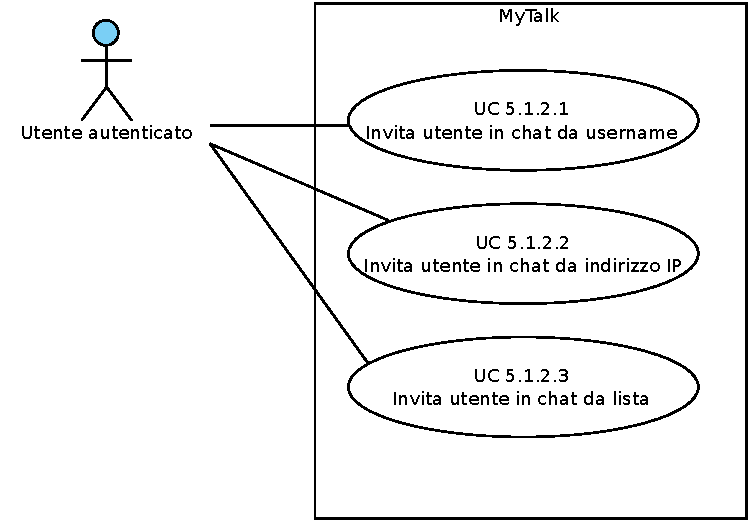
\includegraphics[scale=0.7]{./casi_uso/UC5-1-2.pdf}
\caption{UC 5.1.2 Invia richiesta di comunicazione chat ad utenti.}
\end{figure}

\noindent
\textbf{Attori primari:} utente autenticato.\\
\textbf{Descrizione:} l'utente vuole iniziare una nuova chat, procede quindi con la selezione degli utenti che ne faranno parte e il sistema procede con l'invio della richiesta e la creazione della chat.\\
\textbf{Precondizione:} l'utente vuole iniziare una nuova chat, al momento ci possono essere altre chat attive.\\ 
\textbf{Postcondizione:} l'utente ha selezionato gli utenti che faranno parte della chat, il sistema provvede ad inviare le richieste ai vari utenti e successivamente a creare la chat.\\
\textbf{Scenario principale:}
\begin{itemize}
\item l'utente può selezionare gli utenti tramite username;
\item l'utente può selezionare gli utenti tramite indirizzo IP$_{|g|}$;
\item l'utente può selezionare gli utenti tramite la lista degli utenti registrati al server.
\end{itemize}

\subsubsection{UC 5.1.2.1 Invita utente in chat da username}

\begin{figure}[htbp]
\centering
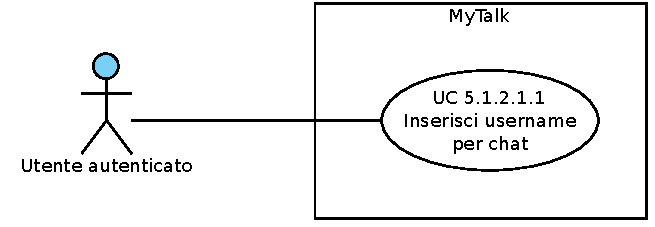
\includegraphics[scale=0.7]{./casi_uso/UC5-1-2-1.pdf}
\caption{UC 5.1.2.1 Invita utente in chat tramite username.}
\end{figure}

\noindent
\textbf{Attori primari:} utente autenticato.\\
\textbf{Descrizione:} l'utente vuole iniziare una nuova chat e vuole selezionare uno o più utenti dallo username.\\
\textbf{Precondizione:} l'utente vuole iniziare una nuova chat scegliendo uno o più utenti dallo username, al momento ci possono essere altre chat attive.\\ 
\textbf{Postcondizione:} l'utente ha aggiunto alla selezione gli utenti che faranno parte della chat individuati tramite username.\\
\textbf{Scenario principale:}
\begin{itemize}
\item l'utente inserisce lo username dell'utente cercato;
\item l'utente a cui corrisponde lo username è stato aggiunto alla lista degli utenti che faranno parte della chat.
\end{itemize}

\subsubsection{UC 5.1.2.1.1 Inserisci username per chat}
\noindent
\textbf{Attori primari:} utente autenticato.\\
\textbf{Descrizione:} l'utente autenticato vuole invitare in chat un altro utente registrato nel sistema conoscendone lo username, quindi inserisce lo username.\\
\textbf{Precondizione:} l'utente è autenticato. Il sistema è funzionante e l'utente vuole invitare in chat un altro utente conoscendone lo username dunque lo inserisce.\\
\textbf{Postcondizione:} lo username è stato inserito.\\
\textbf{Scenario principale:}
\begin{itemize}
\item l'utente inserisce lo username dell'utente che vuole invitare in chat.
\end{itemize}

\subsubsection{UC 5.1.2.2 Invita utente in chat da indirizzo IP$_{|g|}$}

\begin{figure}[htbp]
\centering
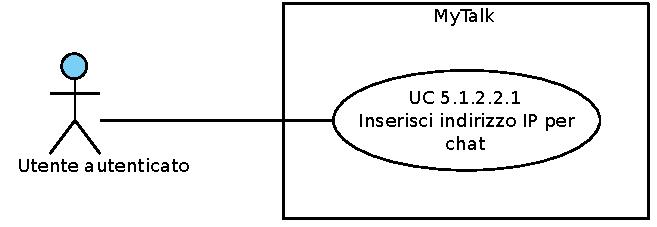
\includegraphics[scale=0.7]{./casi_uso/UC5-1-2-2.pdf}
\caption{UC 5.1.2.2 Invita utente in chat tramite indirizzo IP$_{|g|}$.}
\end{figure}

\noindent
\textbf{Attori primari:} utente autenticato.\\
\textbf{Descrizione:} l'utente vuole iniziare una nuova chat e vuole selezionare uno o più utenti dall'indirizzo IP$_{|g|}$.\\
\textbf{Precondizione:} l'utente vuole iniziare una nuova chat scegliendo uno o più utenti dall'indirizzo IP$_{|g|}$, al momento ci possono essere altre chat attive.\\ 
\textbf{Postcondizione:}  l'utente ha aggiunto alla selezione gli utenti che faranno parte della chat individuati tramite indirizzo IP$_{|g|}$.\\
\textbf{Scenario principale:}
\begin{itemize}
\item l'utente inserisce l'indirizzo IP$_{|g|}$ dell'utente cercato;
\item l'utente a cui corrisponde l'indirizzo IP$_{|g|}$ è stato aggiunto alla lista degli utenti che faranno parte della chat.
\end{itemize}

\subsubsection{UC 5.1.2.2.1 Inserisci indirizzo IP$_{|g|}$ per chat}
\noindent
\textbf{Attori primari:} utente autenticato.\\
\textbf{Descrizione:} l'utente autenticato vuole invitare in chat un altro utente registrato nel sistema conoscendone l'indirizzo IP$_{|g|}$, inserisce quindi l'indirizzo IP$_{|g|}$.\\
\textbf{Precondizione:} l'utente è autenticato. Il sistema è funzionante e l'utente vuole invitare in chat un altro utente conoscendone l'indirizzo IP$_{|g|}$ dunque lo inserisce.\\
\textbf{Postcondizione:} l'indirizzo IP$_{|g|}$ è stato inserito.\\
\textbf{Scenario principale:}
\begin{itemize}
\item l'utente inserisce l'indirizzo IP$_{|g|}$ dell'utente che vuole invitare in chat.
\end{itemize}

\subsubsection{UC 5.1.2.3 Invita utente in chat da lista}

\begin{figure}[htbp]
\centering
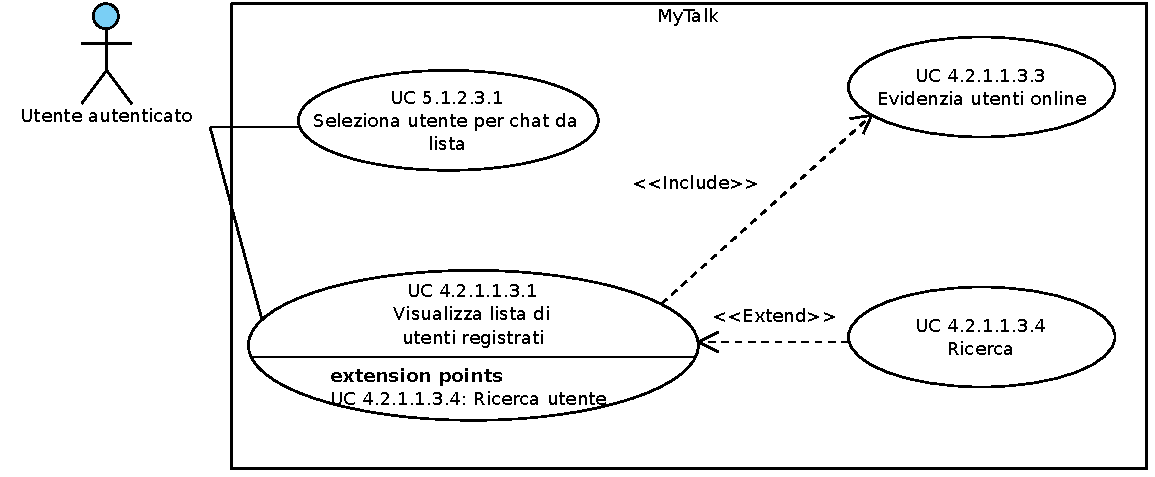
\includegraphics[scale=0.7]{./casi_uso/UC5-1-2-3.pdf}
\caption{UC 5.1.2.3 Invita utente in chat tramite lista.}
\end{figure}

\noindent
\textbf{Attori primari:} utente autenticato.\\
\textbf{Descrizione:} l'utente vuole iniziare una nuova chat e vuole selezionare uno o più utenti dalla lista degli utenti registrati al server.\\
\textbf{Precondizione:} l'utente vuole iniziare una nuova chat scegliendo uno o più utenti dalla lista di utenti registrati al server, al momento ci possono essere altre chat attive.\\ 
\textbf{Postcondizione:}  l'utente ha aggiunto alla selezione gli utenti che faranno parte della chat individuati tramite una selezione dalla lista degli utenti registrati.\\
\textbf{Scenario principale:}
\begin{itemize}
\item l'utente visualizza la lista degli utenti registrati;
%\item l'utente può ricercare nella lista;
\item l'utente seleziona gli utenti che desidera aggiungere alla lista di quelli che formeranno la chat;
\item gli utenti selezionati sono stati aggiunti alla lista che formerà la chat.
\end{itemize}
\textbf{Scenario alternativo:} l'utente effettua una ricerca nella lista degli utenti registrati per trovare l'utente con cui vuole iniziare una conversazione chat.

\subsubsection{UC 5.1.2.3.1 Seleziona utente per chat da lista}
\noindent
\textbf{Attori primari:} utente autenticato.\\
\textbf{Descrizione:} viene visualizzata la lista degli utenti registrati. L'utente può cercarli in essa e può selezionare più di un utente da aggiungere alla lista che poi costituirà gli utenti partecipanti alla chat.\\
\textbf{Precondizione:} l'utente è autenticato. Esso vuole costituire una chat formata da uno o più utenti e vuole selezionarne almeno uno dalla lista degli utenti registrati.\\
\textbf{Postcondizione:} il sistema ha aggiunto gli utenti (possibilmente anche uno solo) alla lista degli utenti che poi costituiranno la chat.\\
\textbf{Scenario principale:}
\begin{itemize}
\item l'utente visualizza la lista degli utenti registrati;
\item gli utenti online vengono evidenziati;
\item l'utente può ricercare in questa lista;
\item l'utente seleziona uno o più utenti da aggiungere alla lista di quelli che formeranno la chat;
\item gli utenti vengono aggiunti alla lista.
\end{itemize}

\subsubsection{UC 5.2 Visualizza chat}
\noindent
\textbf{Attori primari:} utente autenticato.\\
\textbf{Descrizione:} l'utente richiede di visualizzare una chat alla quale lui fa parte.\\
\textbf{Precondizione:} l'utente vuole visualizzare una chat di cui lui fa parte, al momento vi è quindi almeno una chat aperta.\\
\textbf{Postcondizione:} il sistema ha visualizzato la chat richiesta dall'utente.\\
\textbf{Scenario principale:}
\begin{itemize}
\item l'utente richiede di visualizzare una chat;
\item il sistema visualizza la chat richiesta dall'utente.
\end{itemize}


\subsubsection{UC 5.3 Inserisci messaggio}
\noindent
\textbf{Attori primari:} utente autenticato.\\
\textbf{Descrizione:} l'utente autenticato vuole inserire un nuovo messaggio nella chat che ha voluto visualizzare in precedenza.\\
\textbf{Precondizione:} l'utente autenticato vuole inserire un nuovo messaggio all'interno della chat che ha appena visualizzato, una chat è appena stata visualizzata dall'utente.\\
\textbf{Postcondizione:} l'utente autenticato ha inserito un nuovo messaggio testuale, tale messaggio è stato visualizzato all'interno della chat, la chat continua.\\
\textbf{Scenario principale:}
\begin{itemize}
\item l'utente inserisce un nuovo messaggio all'interno della chat appena visualizzata dal sistema;
\item il messaggio inserito dall'utente è visualizzato all'interno della chat.
\end{itemize}

\subsubsection{UC 5.4 Chiudi chat}
\noindent
\textbf{Attori primari:} utente autenticato.\\
\textbf{Descrizione:} l'utente autenticato richiede di terminare una chat di cui fa parte, la chat che verrà chiusa sarà quella attualmente visualizzata.\\
\textbf{Precondizione:} l'utente autenticato vuole uscire dalla chat attualmente visualizzata dal sistema, vi è quindi almeno una chat alla quale l'utente prende parte.\\
\textbf{Postcondizione:} l'utente autenticato è uscito dalla chat visualizzata dal sistema, la chat rimane comunque attiva per gli altri partecipanti alla chiamata.\\
\textbf{Scenario principale:}
\begin{itemize}
\item l'utente richiede di chiudere la chat attualmente visualizzata;
\item la chat attualmente visualizzata viene chiusa.
\end{itemize}

\subsubsection{UC 6 Logout}
\noindent
\textbf{Attori primari:} utente, utente autenticato.\\
\textbf{Descrizione:} l'utente autenticato richiede di terminare la propria sessione e uscire dal sistema diventando nuovamente utente.\\
\textbf{Precondizione:} l'utente autenticato vuole uscire dal sistema.\\
\textbf{Postcondizione:} l'utente autenticato è uscito dal sistema ridiventando utente.\\
\textbf{Scenario principale:}
\begin{itemize}
\item l'utente richiede di terminare la propria sessione;
\item l'utente è uscito dal sistema;
\item l'utente autenticato è diventato utente.
\end{itemize}

\newpage

\subsection{Ambito amministratore}
\subsubsection{UCA 0 Caso base amministratore}

\begin{figure}[htbp]
\centering
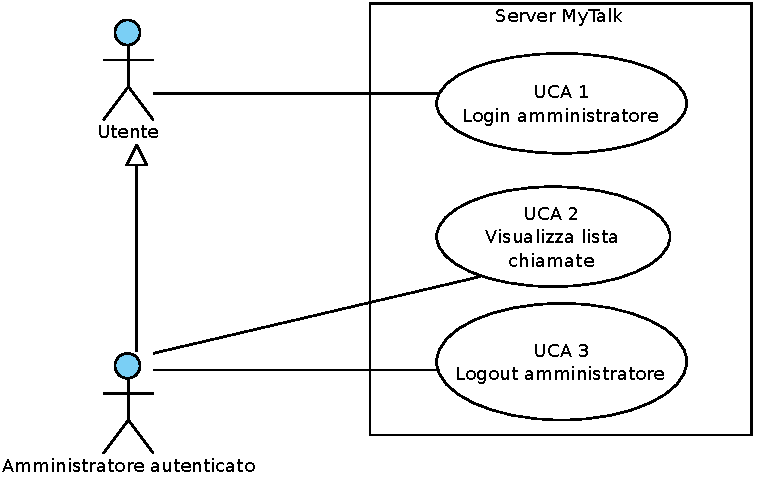
\includegraphics[scale=0.7]{./casi_uso/UCA0.pdf}
\caption{UCA 0 Caso base amministratore.}
\end{figure}

\noindent 
\textbf{Attori principali:} utente, amministratore autenticato.\\
\textbf{Descrizione:} l'utente, appena entrato nella pagina di amministrazione, non è autenticato e può effettuare il login per diventare amministratore autenticato. L'amministratore autenticato può visualizzare e filtrare le chiamate effettuate dagli utenti del sistema e può visualizzare le statistiche relative a queste chiamate, inoltre può effettuare il logout.\\
\textbf{Precondizione:} l'utente non ha ancora effettuato il login, il sistema è funzionante e pronto all'interazione.\\
\textbf{Postcondizione:} l'amministratore autenticato ha visualizzato le statistiche delle chiamate selezionate ed ha effettuato il logout, ritornando utente.\\
\textbf{Scenario principale:}
\begin{itemize}
\item l'utente può effettuare l'autenticazione diventando amministratore autenticato;
\item l'amministratore autenticato può visualizzare e filtrare le chiamate effettuate dagli utenti;
\item l'amministratore autenticato può visualizzare le statistiche delle chiamate selezionate;
\item l'amministratore autenticato può effettuare il logout ritornando utente.
\end{itemize}
\textbf{Scenario alternativo:} le credenziali non risultano corrette, l'utente riceve un opportuno messaggio di avviso da parte del sistema e può eventualmente ritentare il login.

\newpage

\subsubsection{UCA 1 Login amministratore}

\begin{figure}[htbp]
\centering
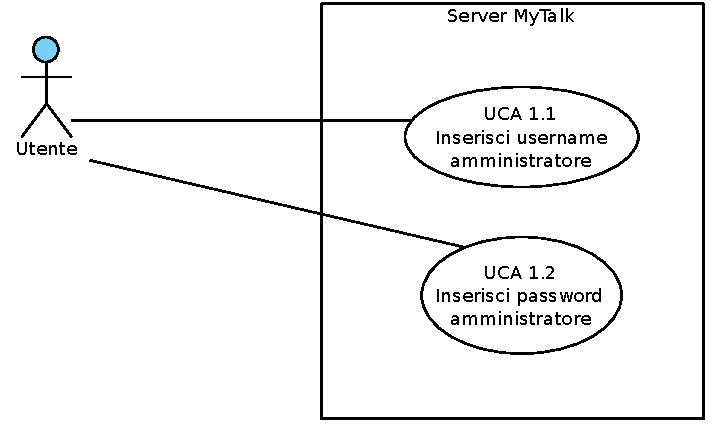
\includegraphics[scale=0.8]{./casi_uso/UCA1.pdf}
\caption{UCA 1 Inserimento credenziali amministratore.}
\end{figure}

\noindent 
\textbf{Attori principali:} utente.\\
\textbf{Descrizione:} l'utente immette le proprie credenziali, se queste risultano corrette l'utente diventa amministratore autenticato.\\
\textbf{Precondizione:} l'utente vuole effettuare il login, e deve inserire le proprie credenziali.\\
\textbf{Postcondizione:} l'utente ha effettuato il login ed è diventato amministratore autenticato.\\
\textbf{Scenario principale:}
\begin{itemize}
\item l'utente inserisce il proprio username;
\item l'utente inserisce la propria password;
\item l'utente ha effettuato il login ed è diventato amministratore autenticato;
\end{itemize}

\subsubsection{UCA 1.1 Inserisci username amministratore}
\noindent
\textbf{Attori primari:} utente.\\
\textbf{Descrizione:} l'utente immette il proprio username.\\
\textbf{Precondizione:} l'utente è pronto ad inserire il proprio username per il login.\\
\textbf{Postcondizione:} l'utente ha immesso il proprio username.\\
\textbf{Scenario principale:}
\begin{itemize}
\item l'utente immette il proprio username.
\end{itemize}

\subsubsection{UCA 1.2 Inserisci password amministratore}
\noindent
\textbf{Attori primari:} utente.\\
\textbf{Descrizione:} l'utente immette la propria password.\\
\textbf{Precondizione:} l'utente è pronto ad inserire la propria password per il login.\\
\textbf{Postcondizione:} l'utente ha immesso la propria password.\\
\textbf{Scenario principale:}
\begin{itemize}
\item l'utente immette la propria password.
\end{itemize}

\newpage

\subsubsection{UCA 2 Visualizza lista chiamate}

\begin{figure}[htbp]
\centering
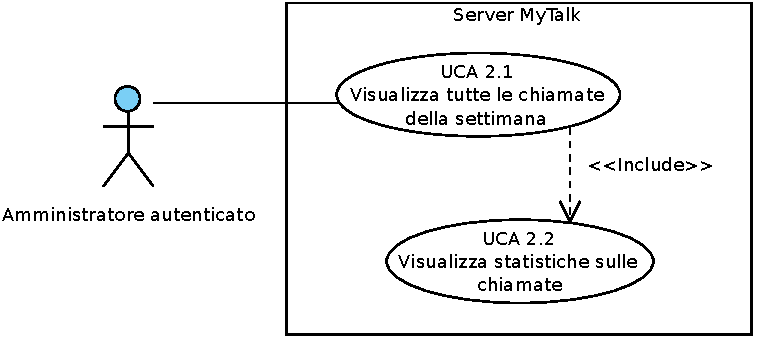
\includegraphics[scale=0.7]{./casi_uso/UCA2.pdf}
\caption{UCA 2 Visualizzazione lista chiamate effettuate dagli utenti.}
\end{figure}

\noindent
\textbf{Attori primari:} amministratore autenticato.\\
\textbf{Descrizione:} l'amministratore autenticato visualizza la lista delle chiamate effettuate dagli utenti nella settimana, può inoltre filtrare le chiamate in base a certi parametri e visualizzare le statistiche relative a queste chiamate.\\
\textbf{Precondizione:} l'amministratore è autenticato. Il server è funzionante. L'amministratore autenticato vuole visualizzare le chiamate effettuate dagli utenti e vedere le relative statistiche.\\
\textbf{Postcondizione:} l'amministratore autenticato ha visualizzato la lista delle chiamate effettuate dagli utenti e ha visualizzato le relative statistiche.\\
\textbf{Scenario principale:}
\begin{itemize}
\item l'amministratore autenticato vede la lista delle chiamate effettuate dagli utenti nella settimana;
\item l'amministratore autenticato può filtrare le chiamate in base a certi parametri;
\item l'amministratore autenticato visualizza le statistiche sulle chiamate;
\end{itemize}

\subsubsection{UCA 2.1 Visualizza tutte le chiamate della settimana}

\begin{figure}[htbp]
\centering
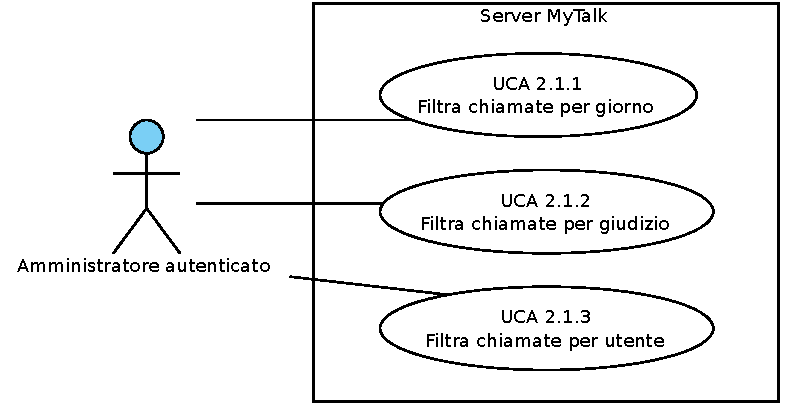
\includegraphics[scale=0.7]{./casi_uso/UCA2-1.pdf}
\caption{UCA 2.1 Visualizzazione lista chiamate settimanali effettuate dagli utenti.}
\end{figure}

\noindent
\textbf{Attori primari:} amministratore autenticato.\\
\textbf{Descrizione:} l'amministratore autenticato visualizza tutte le chiamate effettuate dagli utenti nella settimana, può inoltre filtrare le chiamate in base a certi parametri.\\
\textbf{Precondizione:} l'amministratore è autenticato. Il server è funzionante e l'amministratore autenticato vuole visualizzare le chiamate effettuate dagli utenti.\\
\textbf{Postcondizione:} l'amministratore autenticato ha visualizzato le chiamate effettuate dagli utenti.\\
\textbf{Scenario principale:}
\begin{itemize}
\item l'amministratore autenticato visualizza tutte le chiamate effettuate dagli utenti nella settimana;
\item l'amministratore autenticato può filtrare le chiamate in base a certi parametri;
\end{itemize}

\subsubsection{UCA 2.1.1 Filtra chiamate per giorno}

\begin{figure}[htbp]
\centering
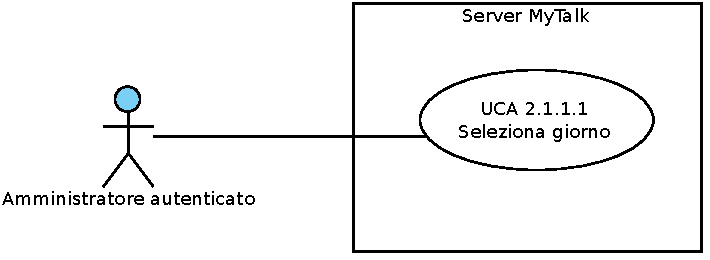
\includegraphics[scale=0.7]{./casi_uso/UCA2-1-1.pdf}
\caption{UCA 2.1.1 Visualizzazione lista chiamate filtrate per giorno.}
\end{figure}

\noindent
\textbf{Attori primari:} amministratore autenticato.\\
\textbf{Descrizione:} l'amministratore autenticato filtra le chiamate degli utenti in base al giorno in cui sono state effettuate.\\
\textbf{Precondizione:} l'amministratore è autenticato. Il server è funzionante e l'amministratore autenticato vuole filtrare le chiamate in base al giorno in cui sono state effettuate.\\
\textbf{Postcondizione:} l'amministratore autenticato ha filtrato le chiamate in base al giorno in cui sono state effettuate.\\
\textbf{Scenario principale:}
\begin{itemize}
\item l'amministratore autenticato seleziona il giorno di cui vuole visualizzare le chiamate effettuate;
\item il sistema restituisce la lista delle chiamate effettuate nel giorno indicato.
\end{itemize}
\textbf{Scenario alternativo:} Nel giorno indicato non sono state effettuate chiamate, l'amministratore autenticato ne riceve debita comunicazione e può poi selezionare un nuovo giorno.\\

\subsubsection{UCA 2.1.1.1 Seleziona giorno}
\noindent
\textbf{Attori primari:} amministratore autenticato.\\
\textbf{Descrizione:} l'amministratore autenticato seleziona il giorno di cui vuole visualizzare le chiamate effettuate.\\
\textbf{Precondizione:} l'amministratore è autenticato. Il server è funzionante e l'amministratore autenticato vuole visualizzare le chiamate effettuate in un certo giorno, dunque seleziona il giorno.\\
\textbf{Postcondizione:} l'amministratore autenticato ha selezionato il giorno di cui visualizzare le chiamate effettuate.\\
\textbf{Scenario principale:}
\begin{itemize}
\item l'amministratore autenticato seleziona il giorno di cui vuole visualizzare le chiamate effettuate.
\end{itemize}

\subsubsection{UCA 2.1.2 Filtra chiamate per giudizio}

\begin{figure}[htbp]
\centering
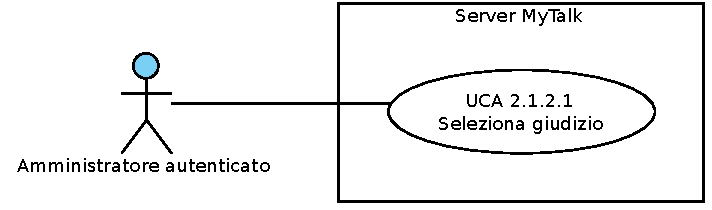
\includegraphics[scale=0.7]{./casi_uso/UCA2-1-2.pdf}
\caption{UCA 2.1.2 Visualizzazione lista chiamate filtrate per giudizio.}
\end{figure}

\noindent
\textbf{Attori primari:} amministratore autenticato.\\
\textbf{Descrizione:} l'amministratore autenticato filtra le chiamate degli utenti in base al giudizio che hanno ricevuto.\\
\textbf{Precondizione:} l'amministratore è autenticato. Il server è funzionante e l'amministratore autenticato vuole filtrare le chiamate in base al giudizio che hanno ricevuto.\\
\textbf{Postcondizione:} l'amministratore autenticato ha filtrato le chiamate in base al giudizio che hanno ricevuto.\\
\textbf{Scenario principale:}
\begin{itemize}
\item l'amministratore autenticato seleziona il giudizio in base al quale vuole visualizzare le chiamate;
\item il sistema restituisce la lista delle chiamate che hanno ricevuto il giudizio selezionato.
\end{itemize}
\textbf{Scenario alternativo:} Nessuna chiamata ha ottenuto il giudizio selezionato, l'amministratore autenticato ne riceve debita comunicazione e può poi selezionare un nuovo giudizio.\\

\subsubsection{UCA 2.1.2.1 Seleziona giudizio}
\noindent
\textbf{Attori primari:} amministratore autenticato.\\
\textbf{Descrizione:} l'amministratore autenticato seleziona il giudizio in base al quale vuole visualizzare le chiamate effettuate.\\
\textbf{Precondizione:} l'amministratore è autenticato. Il server è funzionante e l'amministratore autenticato vuole visualizzare le chiamate effettuate che hanno ricevuto un certo giudizio, dunque seleziona il giudizio.\\
\textbf{Postcondizione:} l'amministratore autenticato ha selezionato il giudizio in base al quale visualizzare le chiamate effettuate.\\
\textbf{Scenario principale:}
\begin{itemize}
\item l'amministratore autenticato seleziona il giudizio in base al quale vuole visualizzare le chiamate effettuate.
\end{itemize}

\subsubsection{UCA 2.1.3 Filtra chiamate per utente}

\begin{figure}[htbp]
\centering
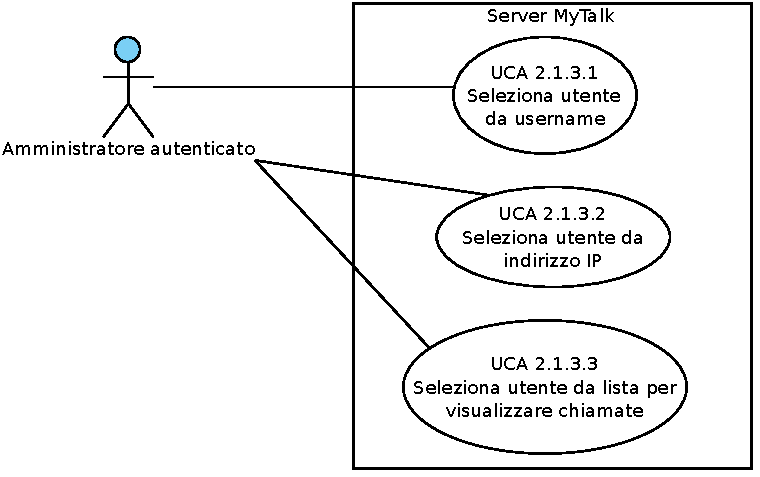
\includegraphics[scale=0.7]{./casi_uso/UCA2-1-3.pdf}
\caption{UCA 2.1.3 Filtra chiamate per utente.}
\end{figure}

\noindent
\textbf{Attori primari:} amministratore autenticato.\\
\textbf{Descrizione:} l'amministratore autenticato filtra le chiamate in base all'utente che vi ha partecipato.\\
\textbf{Precondizione:} l'amministratore è autenticato. Il server è funzionante e l'amministratore autenticato vuole filtrare le chiamate in base all'utente che vi ha partecipato.\\
\textbf{Postcondizione:} l'amministratore autenticato ha filtrato le chiamate in base all'utente che vi ha partecipato.\\
\textbf{Scenario principale:}
\begin{itemize}
\item l'amministratore autenticato seleziona l'utente di cui vuole visualizzare le chiamate a cui ha partecipato;
\item il sistema restituisce la lista delle chiamate a cui ha partecipato l'utente selezionato.
\end{itemize}
\textbf{Scenario alternativo:} L'utente indicato non ha partecipato a chiamate, il sistema ne darà debita comunicazione all'amministratore autenticato che potrà poi selezionare un altro utente.\\

\subsubsection{UCA 2.1.3.1 Seleziona utente da username}

\begin{figure}[htbp]
\centering
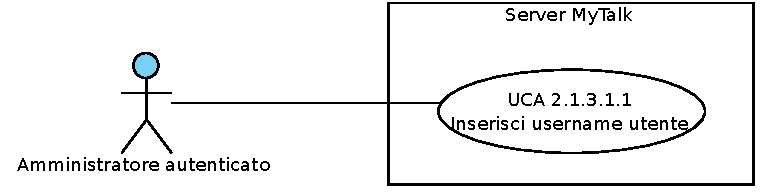
\includegraphics[scale=0.7]{./casi_uso/UCA2-1-3-1.pdf}
\caption{UCA 2.1.3.1 Seleziona utente tramite username per visualizzare chiamate.}
\end{figure}

\noindent
\textbf{Attori primari:} amministratore autenticato.\\
\textbf{Descrizione:} l'amministratore autenticato vuole visualizzare le chiamate a cui ha partecipato un utente di cui conosce lo username, inserisce quindi lo username e il sistema provvederà a visualizzare le chiamate a cui l'utente ha partecipato.\\
\textbf{Precondizione:} l'amministratore è autenticato. Il sistema è funzionante e l'amministratore autenticato vuole visualizzare le chiamate a cui ha partecipato un utente di cui conosce lo username.\\
\textbf{Postcondizione:} l'amministratore autenticato ha selezionato l'utente indicandone lo username.\\
\textbf{Scenario principale:}
\begin{itemize}
\item l'amministratore autenticato inserisce lo username dell'utente di cui vuole visualizzare le chiamate a cui ha partecipato;
\item il sistema, dopo aver appurato che esiste un utente con lo username inserito, filtra la lista delle chiamate in base all'utente corrispondente.
\end{itemize}
\textbf{Scenario alternativo:} lo username inserito dall'amministratore autenticato non corrisponde ad alcun utente iscritto al sistema. All'amministratore autenticato ne viene data opportuna comunicazione, dopodiché avrà la possibilità di ripetere l'operazione.

\subsubsection{UCA 2.1.3.1.1 Inserisci username utente}
\noindent
\textbf{Attori primari:} amministratore autenticato.\\
\textbf{Descrizione:} l'amministratore autenticato vuole visualizzare le chiamate a cui ha partecipato un utente di cui conosce lo username, inserisce quindi lo username.\\
\textbf{Precondizione:} l'amministratore è autenticato. Il sistema è funzionante e l'amministratore autenticato vuole visualizzare le chiamate a cui ha partecipato un utente di cui conosce lo username.\\
\textbf{Postcondizione:} l'amministratore autenticato ha inserito lo username dell'utente di cui vuole visualizzare le chiamate a cui ha partecipato. Il sistema è pronto a filtrare le chiamate.\\
\textbf{Scenario principale:}
\begin{itemize}
\item l'amministratore autenticato inserisce lo username dell'utente di cui vuole visualizzare le chiamate a cui ha partecipato.
\end{itemize}

\subsubsection{UCA 2.1.3.2 Seleziona utente da indirizzo IP$_{|g|}$}

\begin{figure}[htbp]
\centering
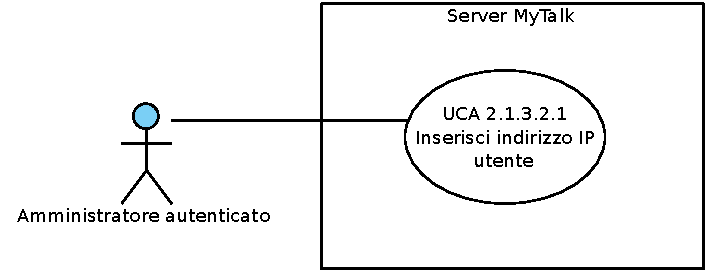
\includegraphics[scale=0.7]{./casi_uso/UCA2-1-3-2.pdf}
\caption{UCA 2.1.3.2 Seleziona utente tramite indirizzo IP$_{|g|}$ per visualizzare chiamate.}
\end{figure}

\noindent
\textbf{Attori primari:} amministratore autenticato.\\
\textbf{Descrizione:} l'amministratore autenticato vuole visualizzare le chiamate a cui ha partecipato un utente di cui conosce l'indirizzo IP$_{|g|}$, inserisce quindi l'indirizzo IP$_{|g|}$ e il sistema provvederà a visualizzare le chiamate a cui l'utente ha partecipato.\\
\textbf{Precondizione:} l'amministratore è autenticato. Il sistema è funzionante e l'amministratore autenticato vuole visualizzare le chiamate a cui ha partecipato un utente di cui conosce l'indirizzo IP$_{|g|}$.\\
\textbf{Postcondizione:} l'amministratore autenticato ha selezionato l'utente indicandone l'indirizzo IP$_{|g|}$.\\
\textbf{Scenario principale:}
\begin{itemize}
\item l'amministratore autenticato inserisce l'indirizzo IP$_{|g|}$ dell'utente di cui vuole visualizzare le chiamate a cui ha partecipato;
\item il sistema, dopo aver appurato che esiste un utente con l'indirizzo IP$_{|g|}$ inserito, filtra la lista delle chiamate in base all'utente corrispondente.
\end{itemize}
\textbf{Scenario alternativo:} l'indirizzo IP$_{|g|}$ inserito dall'amministratore autenticato non corrisponde ad alcun utente iscritto al sistema. All'amministratore autenticato ne viene data opportuna comunicazione, dopodiché avrà la possibilità di ripetere l'operazione.

\subsubsection{UCA 2.1.3.2.1 Inserisci indirizzo IP$_{|g|}$ utente}
\noindent
\textbf{Attori primari:} amministratore autenticato.\\
\textbf{Descrizione:} l'amministratore autenticato vuole visualizzare le chiamate a cui ha partecipato un utente di cui conosce l'indirizzo IP$_{|g|}$, inserisce quindi l'indirizzo IP$_{|g|}$.\\
\textbf{Precondizione:} l'amministratore è autenticato. Il sistema è funzionante e l'amministratore autenticato vuole visualizzare le chiamate a cui ha partecipato un utente di cui conosce l'indirizzo IP$_{|g|}$, dunque lo inserisce.\\
\textbf{Postcondizione:} l'amministratore autenticato ha inserito l'indirizzo IP$_{|g|}$ dell'utente di cui vuole visualizzare le chiamate a cui ha partecipato. Il sistema è pronto a filtrare le chiamate.\\
\textbf{Scenario principale:}
\begin{itemize}
\item l'amministratore autenticato inserisce l'indirizzo IP$_{|g|}$ dell'utente di cui vuole visualizzare le chiamate a cui ha partecipato.
\end{itemize}

\newpage

\subsubsection{UCA 2.1.3.3 Seleziona utente da lista per visualizzare chiamate}

\begin{figure}[htbp]
\centering
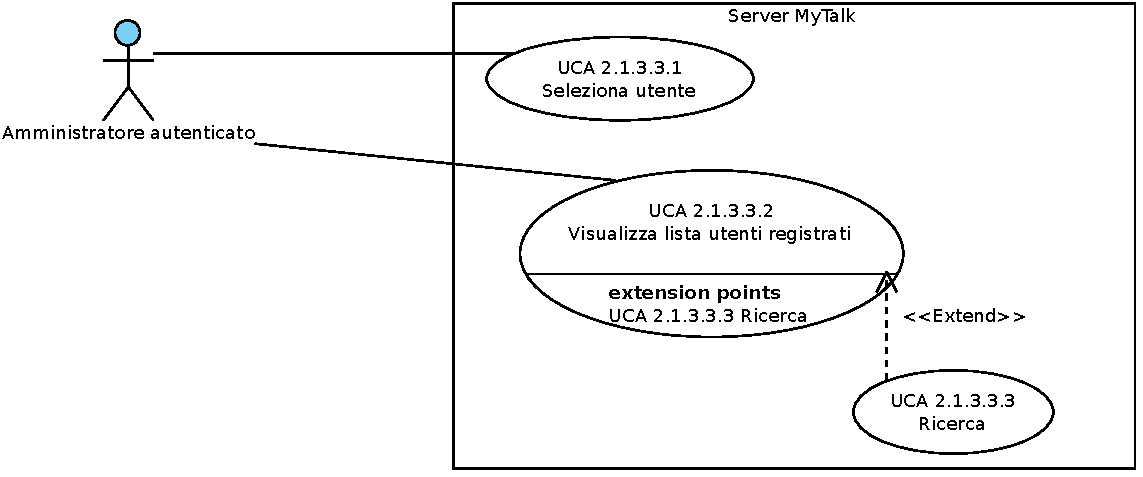
\includegraphics[scale=0.7]{./casi_uso/UCA2-1-3-3.pdf}
\caption{UCA 2.1.3.3 Seleziona utente tramite lista per visualizzare chiamate.}
\end{figure}

\noindent
\textbf{Attori primari:} amministratore autenticato.\\
\textbf{Descrizione:} l'amministratore autenticato vuole selezionare un utente dalla lista degli utenti registrati per visualizzare le chiamate a cui ha partecipato. L'amministratore autenticato visualizza la lista e sceglie l'utente di cui desidera visualizzare le chiamate.\\%, eventualmente dopo averlo ricercato.\\
\textbf{Precondizione:} l'amministratore è autenticato. Il sistema è funzionante e l'amministratore vuole selezionare un utente, dalla lista degli utenti registrati, per visualizzare le chiamate a cui ha partecipato.\\
\textbf{Postcondizione:} l'amministratore autenticato ha selezionato l'utente dalla lista. \\
\textbf{Scenario principale:}
\begin{itemize}
\item l'amministratore autenticato visualizza la lista degli utenti registrati;
%\item l'amministratore autenticato può ricercare nella lista un utente;
\item l'amministratore autenticato seleziona l'utente di cui desidera visualizzare le chiamate a cui ha partecipato;
\item il sistema filtra la lista delle chiamate in base all'utente selezionato.
\end{itemize}
\textbf{Scenario alternativo:} l'amministratore autenticato effettua una ricerca nella lista degli utenti registrati per trovare l'utente di cui vuole visualizzare le chiamate.

\subsubsection{UCA 2.1.3.3.1 Seleziona utente}

\noindent
\textbf{Attori primari:} amministratore autenticato.\\
\textbf{Descrizione:} viene visualizzata la lista degli utenti registrati. L'amministratore autenticato può cercare utenti nella lista e può selezionare un solo utente.\\
\textbf{Precondizione:} l'amministratore è autenticato. Il sistema è funzionante e l'amministratore autenticato vuole selezionare un utente dalla lista degli utenti registrati per visualizzare le chiamate a cui ha partecipato.\\
\textbf{Postcondizione:} l'amministratore autenticato ha selezionato l'utente dalla lista.\\
\textbf{Scenario principale:}
\begin{itemize}
\item l'amministratore autenticato seleziona dalla lista l'utente, eventualmente dopo averlo ricercato;
\end{itemize}

\subsubsection{UCA 2.1.3.3.2 Visualizza lista utenti registrati}
\noindent
\textbf{Attori primari:} amministratore autenticato.\\
\textbf{Descrizione:} l'amministratore autenticato vuole selezionare un utente dalla lista degli utenti registrati, che può visualizzare.\\% e nella quale, se lo richiede, può ricercare un utente sulla base dello username o sulla base dell'indirizzo IP$_{|g|}$.\\
\textbf{Precondizione:} l'amministratore è autenticato. Il sistema è funzionante e l'amministratore autenticato vuole selezionare un utente dalla lista degli utenti registrati.\\
\textbf{Postcondizione:} il sistema mostra all'amministratore autenticato la lista degli utenti registrati e permette, su apposita richiesta da parte dell'amministratore autenticato, la ricerca all'interno della lista.\\
\textbf{Scenario principale:}
\begin{itemize}
\item l'amministratore autenticato visualizza la lista degli utenti registrati al sistema;
\item l'amministratore autenticato può ricercare in questa lista.
\end{itemize}
\textbf{Scenario alternativo:} l'amministratore autenticato effettua una ricerca, sulla base dello username o sulla base dell'indirizzo IP$_{|g|}$, nella lista degli utenti registrati per trovare l'utente di cui vuole visualizzare le chiamate.

\subsubsection{UCA 2.1.3.3.3 Ricerca}

\begin{figure}[htbp]
\centering
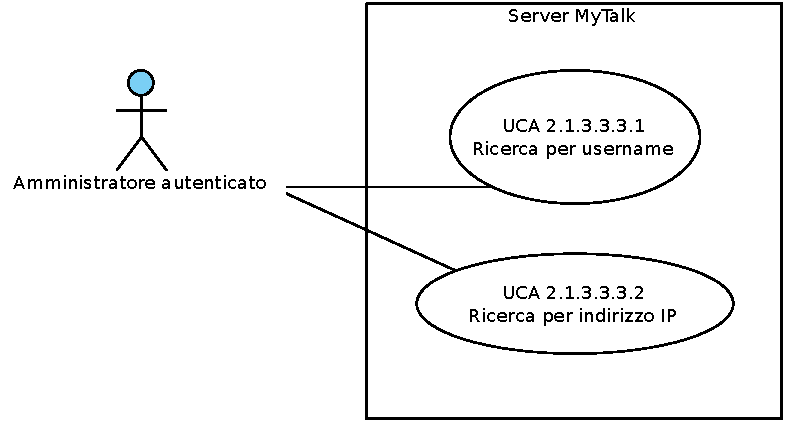
\includegraphics[scale=0.7]{./casi_uso/UCA2-1-3-3-3.pdf}
\caption{UCA 2.1.3.3.3 Ricerca di un utente all'interno della lista degli utenti registrati per visualizzare chiamate.}
\end{figure}

\noindent
\textbf{Attori primari:} amministratore autenticato.\\
\textbf{Descrizione:} l'amministratore autenticato può cercare un utente presente nella lista senza doverla scorrere indicandone lo username o l'indirizzo IP$_{|g|}$.\\
\textbf{Precondizione:} l'amministratore autenticato vuole cercare un utente nella lista senza scorrerla.\\
\textbf{Postcondizione:} il sistema ha visualizzato i risultati della ricerca.\\
\textbf{Scenario principale:}
\begin{itemize}
\item l'amministratore autenticato inserisce lo username o l'indirizzo IP$_{|g|}$ dell'utente cercato;
\item l'amministratore autenticato visualizza i risultati della ricerca e può selezionare l'utente trovato.
\end{itemize}
\textbf{Scenario alternativo:} nessun utente viene trovato, quindi l'amministratore autenticato riceve debita comunicazione e poi può ripetere la ricerca.

\subsubsection{UCA 2.1.3.3.3.1 Ricerca per username}
\noindent
\textbf{Attori primari:} amministratore autenticato.\\
\textbf{Descrizione:} l'amministratore autenticato cerca un utente presente nella lista senza doverla scorrere indicandone lo username.\\
\textbf{Precondizione:} l'amministratore autenticato vuole cercare un utente nella lista degli utenti registrati.\\
\textbf{Postcondizione:} il sistema ha mostrato i risultati della ricerca.\\
\textbf{Scenario principale:}
\begin{itemize}
\item l'amministratore autenticato inserisce lo username dell'utente cercato;
\item l'amministratore autenticato visualizza il risultato della ricerca.
\end{itemize}
\textbf{Scenario alternativo:} nessun utente viene trovato, quindi l'amministratore autenticato riceve debita comunicazione e poi può ripeterla.

\subsubsection{UCA 2.1.3.3.3.2 Ricerca per indirizzo IP$_{|g|}$}
\noindent
\textbf{Attori primari:} amministratore autenticato.\\
\textbf{Descrizione:} l'amministratore autenticato cerca un utente presente nella lista, senza così doverla scorrere, indicandone l'indirizzo IP$_{|g|}$.\\
\textbf{Precondizione:} l'amministratore autenticato vuole cercare un utente nella lista senza scorrerla.\\
\textbf{Postcondizione:} il sistema ha mostrato i risultati della ricerca.\\
\textbf{Scenario principale:}
\begin{itemize}
\item l'amministratore autenticato inserisce l'indirizzo IP$_{|g|}$ dell'utente cercato;
\item l'amministratore autenticato visualizza il risultato della ricerca.
\end{itemize}
\textbf{Scenario alternativo:} nessun utente viene trovato, l'amministratore autenticato riceve debita comunicazione e può ripetere la ricerca.

\newpage

\subsubsection{UCA 2.2 Visualizza statistiche sulle chiamate}

\begin{figure}[htbp]
\centering
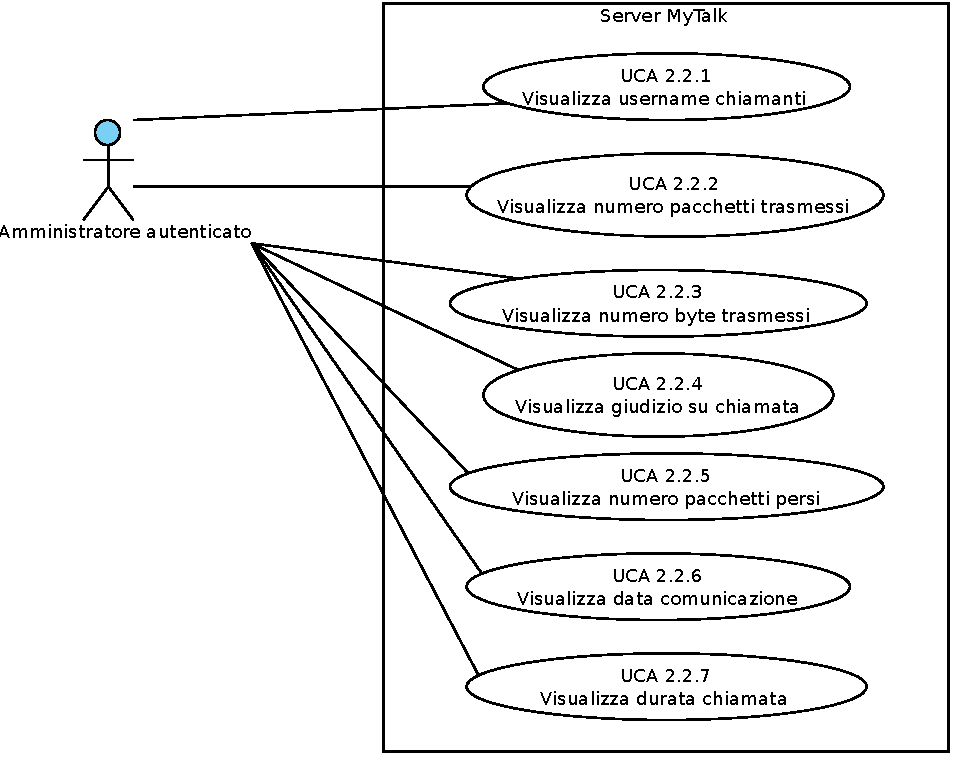
\includegraphics[scale=0.7]{./casi_uso/UCA2-2.pdf}
\caption{UCA 2.2 Visualizzazione delle statistiche relative alle chiamate effettuate dagli utenti.}
\end{figure}

\noindent 
\textbf{Attori primari:} amministratore autenticato.\\
\textbf{Descrizione:} l'amministratore autenticato visualizza le statistiche sulle chiamate e le relative valutazioni degli utenti.\\
\textbf{Precondizione:} il sistema è funzionante e l'amministratore autenticato vuole visualizzare le statistiche sulle chiamate e le relative valutazioni degli utenti.\\
\textbf{Postcondizione:} le statistiche sulle chiamate e le relative valutazioni sono state visualizzate.\\
\textbf{Scenario principale:}
\begin{itemize}
\item l'amministratore autenticato può visualizzare gli username delle persone che hanno partecipato alla chiamata;
\item l'amministratore autenticato può visualizzare il numero di pacchetti trasmessi durante la chiamata;
\item l'amministratore autenticato può visualizzare la quantità di byte trasmessi durante la chiamata;
\item l'amministratore autenticato può visualizzare il giudizio degli utenti su una certa chiamata;
\item l'amministratore autenticato può visualizzare il numero di pacchetti persi durante la chiamata;
\item l'amministratore autenticato può visualizzare la data in cui è stata effettuata la chiamata;
\item l'amministratore autenticato può visualizzare la durata della chiamata.
\end{itemize}

\subsubsection{UCA 2.2.1 Visualizza username chiamanti}
\noindent 
\textbf{Attori primari:} amministratore autenticato.\\
\textbf{Descrizione:} l'amministratore autenticato visualizza gli username degli utenti che hanno partecipato alla chiamata.\\
\textbf{Precondizione:} l'amministratore autenticato vuole visualizzare le statistiche ricevute dagli utenti iscritti.\\
\textbf{Postcondizione:} l'amministratore autenticato ha visualizzato gli username degli utenti che hanno partecipato alla chiamata.\\
\textbf{Scenario principale:}
\begin{itemize}
\item l'amministratore autenticato visualizza gli username degli utenti che hanno partecipato alla chiamata.
\end{itemize}

\subsubsection{UCA 2.2.2 Visualizza numero pacchetti trasmessi}
\noindent 
\textbf{Attori primari:} amministratore autenticato.\\
\textbf{Descrizione:} l'amministratore autenticato visualizza il numero di pacchetti trasmessi durante la chiamata.\\
\textbf{Precondizione:} l'amministratore autenticato vuole visualizzare le statistiche ricevute dagli utenti iscritti.\\
\textbf{Postcondizione:} l'amministratore autenticato ha visualizzato il numero di pacchetti trasmessi durante la chiamata.\\
\textbf{Scenario principale:}
\begin{itemize}
\item l'amministratore autenticato visualizza il numero di pacchetti trasmessi durante la chiamata.
\end{itemize}

\subsubsection{UCA 2.2.3 Visualizza numero byte trasmessi}
\noindent 
\textbf{Attori primari:} amministratore autenticato.\\
\textbf{Descrizione:} l'amministratore autenticato visualizza il numero di byte trasmessi durante la chiamata.\\
\textbf{Precondizione:} l'amministratore autenticato vuole visualizzare le statistiche ricevute dagli utenti iscritti.\\
\textbf{Postcondizione:} l'amministratore autenticato ha visualizzato il numero di byte trasmessi durante la chiamata.\\
\textbf{Scenario principale:}
\begin{itemize}
\item l'amministratore autenticato visualizza la quantità di byte trasmessi durante la chiamata.
\end{itemize}

\subsubsection{UCA 2.2.4 Visualizza giudizio su chiamata}
\noindent 
\textbf{Attori primari:} amministratore autenticato.\\
\textbf{Descrizione:} l'amministratore autenticato visualizza il giudizio degli utenti partecipanti alla chiamata riguardo alla qualità della comunicazione.\\
\textbf{Precondizione:} l'amministratore autenticato vuole visualizzare le statistiche ricevute dagli utenti iscritti.\\
\textbf{Postcondizione:} l'amministratore autenticato ha visualizzato il giudizio degli utenti.\\
\textbf{Scenario principale:}
\begin{itemize}
\item l'amministratore autenticato visualizza il giudizio degli utenti relativi alla qualità della comunicazione.
\end{itemize}

\subsubsection{UCA 2.2.5 Visualizza numero pacchetti persi}
\noindent 
\textbf{Attori primari:} amministratore autenticato.\\
\textbf{Descrizione:} l'amministratore autenticato visualizza il numero di pacchetti persi  durante la chiamata.\\
\textbf{Precondizione:} l'amministratore autenticato vuole visualizzare le statistiche ricevute dagli utenti iscritti.\\
\textbf{Postcondizione:} l'amministratore autenticato ha visualizzato il numero di pacchetti persi durante la chiamata.\\
\textbf{Scenario principale:}
\begin{itemize}
\item l'amministratore autenticato visualizza il numero di pacchetti persi durante la chiamata.
\end{itemize}

\subsubsection{UCA 2.2.6 Visualizza data comunicazione}
\noindent 
\textbf{Attori primari:} amministratore autenticato.\\
\textbf{Descrizione:} l'amministratore autenticato visualizza la data in cui è stata effettuata la chiamata.\\
\textbf{Precondizione:} l'amministratore autenticato vuole visualizzare le statistiche ricevute dagli utenti iscritti.\\
\textbf{Postcondizione:} l'amministratore autenticato ha visualizzato la data in cui è stata effettuata la chiamata.\\
\textbf{Scenario principale:}
\begin{itemize}
\item l'amministratore autenticato visualizza la data in cui è stata effettuata la chiamata.
\end{itemize}

\subsubsection{UCA 2.2.7 Visualizza durata chiamata}
\noindent 
\textbf{Attori primari:} amministratore autenticato.\\
\textbf{Descrizione:} l'amministratore autenticato visualizza la durata della chiamata.\\
\textbf{Precondizione:} l'amministratore autenticato vuole visualizzare le statistiche ricevute dagli utenti iscritti.\\
\textbf{Postcondizione:} l'amministratore autenticato ha visualizzato la durata della chiamata.\\
\textbf{Scenario principale:}
\begin{itemize}
\item l'amministratore autenticato visualizza la durata della chiamata.
\end{itemize}

\subsubsection{UCA 3 Logout amministratore}
\noindent 
\textbf{Attori principali:} utente, amministratore autenticato.\\
\textbf{Descrizione:} l'amministratore autenticato effettua il logout diventando utente.\\
\textbf{Precondizione:} l'amministratore autenticato vuole effettuare il logout.\\
\textbf{Postcondizione:} l'amministratore autenticato ha effettuato il logout ed è diventato utente.\\
\textbf{Scenario principale:}
\begin{itemize}
\item l'amministratore autenticato effettua il logout.
\end{itemize}